\documentclass[twoside]{book}

% Packages required by doxygen
\usepackage{fixltx2e}
\usepackage{calc}
\usepackage{doxygen}
\usepackage[export]{adjustbox} % also loads graphicx
\usepackage{graphicx}
\usepackage[utf8]{inputenc}
\usepackage{makeidx}
\usepackage{multicol}
\usepackage{multirow}
\PassOptionsToPackage{warn}{textcomp}
\usepackage{textcomp}
\usepackage[nointegrals]{wasysym}
\usepackage[table]{xcolor}

% Font selection
\usepackage[T1]{fontenc}
\usepackage[scaled=.90]{helvet}
\usepackage{courier}
\usepackage{amssymb}
\usepackage{sectsty}
\renewcommand{\familydefault}{\sfdefault}
\allsectionsfont{%
  \fontseries{bc}\selectfont%
  \color{darkgray}%
}
\renewcommand{\DoxyLabelFont}{%
  \fontseries{bc}\selectfont%
  \color{darkgray}%
}
\newcommand{\+}{\discretionary{\mbox{\scriptsize$\hookleftarrow$}}{}{}}

% Page & text layout
\usepackage{geometry}
\geometry{%
  a4paper,%
  top=2.5cm,%
  bottom=2.5cm,%
  left=2.5cm,%
  right=2.5cm%
}
\tolerance=750
\hfuzz=15pt
\hbadness=750
\setlength{\emergencystretch}{15pt}
\setlength{\parindent}{0cm}
\setlength{\parskip}{3ex plus 2ex minus 2ex}
\makeatletter
\renewcommand{\paragraph}{%
  \@startsection{paragraph}{4}{0ex}{-1.0ex}{1.0ex}{%
    \normalfont\normalsize\bfseries\SS@parafont%
  }%
}
\renewcommand{\subparagraph}{%
  \@startsection{subparagraph}{5}{0ex}{-1.0ex}{1.0ex}{%
    \normalfont\normalsize\bfseries\SS@subparafont%
  }%
}
\makeatother

% Headers & footers
\usepackage{fancyhdr}
\pagestyle{fancyplain}
\fancyhead[LE]{\fancyplain{}{\bfseries\thepage}}
\fancyhead[CE]{\fancyplain{}{}}
\fancyhead[RE]{\fancyplain{}{\bfseries\leftmark}}
\fancyhead[LO]{\fancyplain{}{\bfseries\rightmark}}
\fancyhead[CO]{\fancyplain{}{}}
\fancyhead[RO]{\fancyplain{}{\bfseries\thepage}}
\fancyfoot[LE]{\fancyplain{}{}}
\fancyfoot[CE]{\fancyplain{}{}}
\fancyfoot[RE]{\fancyplain{}{\bfseries\scriptsize Generated by Doxygen }}
\fancyfoot[LO]{\fancyplain{}{\bfseries\scriptsize Generated by Doxygen }}
\fancyfoot[CO]{\fancyplain{}{}}
\fancyfoot[RO]{\fancyplain{}{}}
\renewcommand{\footrulewidth}{0.4pt}
\renewcommand{\chaptermark}[1]{%
  \markboth{#1}{}%
}
\renewcommand{\sectionmark}[1]{%
  \markright{\thesection\ #1}%
}

% Indices & bibliography
\usepackage{natbib}
\usepackage[titles]{tocloft}
\setcounter{tocdepth}{3}
\setcounter{secnumdepth}{5}
\makeindex

% Hyperlinks (required, but should be loaded last)
\usepackage{ifpdf}
\ifpdf
  \usepackage[pdftex,pagebackref=true]{hyperref}
\else
  \usepackage[ps2pdf,pagebackref=true]{hyperref}
\fi
\hypersetup{%
  colorlinks=true,%
  linkcolor=blue,%
  citecolor=blue,%
  unicode%
}

% Custom commands
\newcommand{\clearemptydoublepage}{%
  \newpage{\pagestyle{empty}\cleardoublepage}%
}

\usepackage{caption}
\captionsetup{labelsep=space,justification=centering,font={bf},singlelinecheck=off,skip=4pt,position=top}

%===== C O N T E N T S =====

\begin{document}

% Titlepage & ToC
\hypersetup{pageanchor=false,
             bookmarksnumbered=true,
             pdfencoding=unicode
            }
\pagenumbering{roman}
\begin{titlepage}
\vspace*{7cm}
\begin{center}%
{\Large Envi\+Nav \\[1ex]\large 1.\+0 }\\
\vspace*{1cm}
{\large Generated by Doxygen 1.8.11}\\
\end{center}
\end{titlepage}
\clearemptydoublepage
\tableofcontents
\clearemptydoublepage
\pagenumbering{arabic}
\hypersetup{pageanchor=true}

%--- Begin generated contents ---
\chapter{Hierarchical Index}
\section{Class Hierarchy}
This inheritance list is sorted roughly, but not completely, alphabetically\+:\begin{DoxyCompactList}
\item Base\+Global\+Planner\begin{DoxyCompactList}
\item \contentsline{section}{R\+R\+T\+Planner}{\pageref{classRRTPlanner}}{}
\end{DoxyCompactList}
\item \contentsline{section}{Map\+Build}{\pageref{classMapBuild}}{}
\item \contentsline{section}{R\+R\+T\+Planner\+Helper\+:\+:q\+Tree}{\pageref{structRRTPlannerHelper_1_1qTree}}{}
\item \contentsline{section}{R\+R\+T\+Planner\+Helper}{\pageref{classRRTPlannerHelper}}{}
\item \contentsline{section}{R\+R\+T\+Planner\+Tester}{\pageref{classRRTPlannerTester}}{}
\end{DoxyCompactList}

\chapter{Class Index}
\section{Class List}
Here are the classes, structs, unions and interfaces with brief descriptions\+:\begin{DoxyCompactList}
\item\contentsline{section}{\hyperlink{classMapBuild}{Map\+Build} }{\pageref{classMapBuild}}{}
\item\contentsline{section}{\hyperlink{structRRTPlannerHelper_1_1qTree}{R\+R\+T\+Planner\+Helper\+::q\+Tree} \\*Structure that holds the data related to each node in the tree }{\pageref{structRRTPlannerHelper_1_1qTree}}{}
\item\contentsline{section}{\hyperlink{classRRTPlanner}{R\+R\+T\+Planner} }{\pageref{classRRTPlanner}}{}
\item\contentsline{section}{\hyperlink{classRRTPlannerHelper}{R\+R\+T\+Planner\+Helper} }{\pageref{classRRTPlannerHelper}}{}
\item\contentsline{section}{\hyperlink{classRRTPlannerTester}{R\+R\+T\+Planner\+Tester} }{\pageref{classRRTPlannerTester}}{}
\end{DoxyCompactList}

\chapter{File Index}
\section{File List}
Here is a list of all documented files with brief descriptions\+:\begin{DoxyCompactList}
\item\contentsline{section}{/home/sammie/catkin\+\_\+ws/src/envi\+\_\+nav/include/\hyperlink{MapBuild_8h}{Map\+Build.\+h} \\*Saves the map generated by the navigation demo }{\pageref{MapBuild_8h}}{}
\item\contentsline{section}{/home/sammie/catkin\+\_\+ws/src/envi\+\_\+nav/include/\hyperlink{RRTPlanner_8h}{R\+R\+T\+Planner.\+h} \\*Global path planner implementing the R\+RT algorithm }{\pageref{RRTPlanner_8h}}{}
\item\contentsline{section}{/home/sammie/catkin\+\_\+ws/src/envi\+\_\+nav/include/\hyperlink{RRTPlannerHelper_8h}{R\+R\+T\+Planner\+Helper.\+h} \\*Global path planner implementing the R\+RT algorithm }{\pageref{RRTPlannerHelper_8h}}{}
\item\contentsline{section}{/home/sammie/catkin\+\_\+ws/src/envi\+\_\+nav/src/\hyperlink{MapBuild_8cpp}{Map\+Build.\+cpp} \\*Saves the map generated by the navigation demo }{\pageref{MapBuild_8cpp}}{}
\item\contentsline{section}{/home/sammie/catkin\+\_\+ws/src/envi\+\_\+nav/src/\hyperlink{mapping__demo_8cpp}{mapping\+\_\+demo.\+cpp} \\*Gives instructions for building the navigation map }{\pageref{mapping__demo_8cpp}}{}
\item\contentsline{section}{/home/sammie/catkin\+\_\+ws/src/envi\+\_\+nav/src/\hyperlink{RRTPlanner_8cpp}{R\+R\+T\+Planner.\+cpp} \\*Global path planner implementing the R\+RT algorithm }{\pageref{RRTPlanner_8cpp}}{}
\item\contentsline{section}{/home/sammie/catkin\+\_\+ws/src/envi\+\_\+nav/src/\hyperlink{RRTPlannerHelper_8cpp}{R\+R\+T\+Planner\+Helper.\+cpp} \\*Global path planner implementing the R\+RT algorithm }{\pageref{RRTPlannerHelper_8cpp}}{}
\item\contentsline{section}{/home/sammie/catkin\+\_\+ws/src/envi\+\_\+nav/test/\hyperlink{EnviNavTests_8cpp}{Envi\+Nav\+Tests.\+cpp} \\*Tests for R\+RT Planning algorithm }{\pageref{EnviNavTests_8cpp}}{}
\end{DoxyCompactList}

\chapter{Class Documentation}
\hypertarget{classMapBuild}{}\section{Map\+Build Class Reference}
\label{classMapBuild}\index{Map\+Build@{Map\+Build}}
\subsection*{Public Member Functions}
\begin{DoxyCompactItemize}
\item 
\hyperlink{classMapBuild_a116a872478f708f37d45bb56f17d1549}{Map\+Build} ()\hypertarget{classMapBuild_a116a872478f708f37d45bb56f17d1549}{}\label{classMapBuild_a116a872478f708f37d45bb56f17d1549}

\begin{DoxyCompactList}\small\item\em The default constructor for the \hyperlink{classMapBuild}{Map\+Build} class. \end{DoxyCompactList}\item 
void \hyperlink{classMapBuild_a6f719b1f109486779ff0d60cc8d7ca45}{save\+\_\+map} ()\hypertarget{classMapBuild_a6f719b1f109486779ff0d60cc8d7ca45}{}\label{classMapBuild_a6f719b1f109486779ff0d60cc8d7ca45}

\begin{DoxyCompactList}\small\item\em Saves the map being built by the navigation demo. \end{DoxyCompactList}\end{DoxyCompactItemize}


The documentation for this class was generated from the following files\+:\begin{DoxyCompactItemize}
\item 
/home/sammie/catkin\+\_\+ws/src/envi\+\_\+nav/include/\hyperlink{MapBuild_8h}{Map\+Build.\+h}\item 
/home/sammie/catkin\+\_\+ws/src/envi\+\_\+nav/src/\hyperlink{MapBuild_8cpp}{Map\+Build.\+cpp}\end{DoxyCompactItemize}

\hypertarget{structRRTPlannerHelper_1_1qTree}{}\section{R\+R\+T\+Planner\+Helper\+:\+:q\+Tree Struct Reference}
\label{structRRTPlannerHelper_1_1qTree}\index{R\+R\+T\+Planner\+Helper\+::q\+Tree@{R\+R\+T\+Planner\+Helper\+::q\+Tree}}


Structure that holds the data related to each node in the tree.  




{\ttfamily \#include $<$R\+R\+T\+Planner\+Helper.\+h$>$}

\subsection*{Public Attributes}
\begin{DoxyCompactItemize}
\item 
geometry\+\_\+msgs\+::\+Pose\+Stamped {\bfseries q}\hypertarget{structRRTPlannerHelper_1_1qTree_afe0b03af9e2d1fbf0a71207303a99dd0}{}\label{structRRTPlannerHelper_1_1qTree_afe0b03af9e2d1fbf0a71207303a99dd0}

\item 
geometry\+\_\+msgs\+::\+Pose\+Stamped {\bfseries q\+Near}\hypertarget{structRRTPlannerHelper_1_1qTree_ab45c90035886f2862897e6ace143e124}{}\label{structRRTPlannerHelper_1_1qTree_ab45c90035886f2862897e6ace143e124}

\item 
int {\bfseries my\+Index}\hypertarget{structRRTPlannerHelper_1_1qTree_a94fbaf1d1f0bda6456755d120156b5c5}{}\label{structRRTPlannerHelper_1_1qTree_a94fbaf1d1f0bda6456755d120156b5c5}

\item 
int {\bfseries near\+Index}\hypertarget{structRRTPlannerHelper_1_1qTree_a47ba5cc49b37e19fcff618edc82f54a5}{}\label{structRRTPlannerHelper_1_1qTree_a47ba5cc49b37e19fcff618edc82f54a5}

\end{DoxyCompactItemize}


\subsection{Detailed Description}
Structure that holds the data related to each node in the tree. 

The documentation for this struct was generated from the following file\+:\begin{DoxyCompactItemize}
\item 
/home/sammie/catkin\+\_\+ws/src/envi\+\_\+nav/include/\hyperlink{RRTPlannerHelper_8h}{R\+R\+T\+Planner\+Helper.\+h}\end{DoxyCompactItemize}

\hypertarget{classRRTPlanner}{}\section{R\+R\+T\+Planner Class Reference}
\label{classRRTPlanner}\index{R\+R\+T\+Planner@{R\+R\+T\+Planner}}


Inheritance diagram for R\+R\+T\+Planner\+:\nopagebreak
\begin{figure}[H]
\begin{center}
\leavevmode
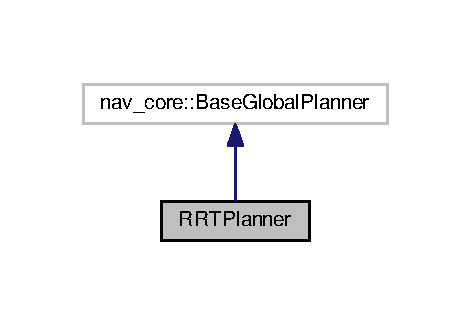
\includegraphics[width=226pt]{classRRTPlanner__inherit__graph}
\end{center}
\end{figure}


Collaboration diagram for R\+R\+T\+Planner\+:\nopagebreak
\begin{figure}[H]
\begin{center}
\leavevmode
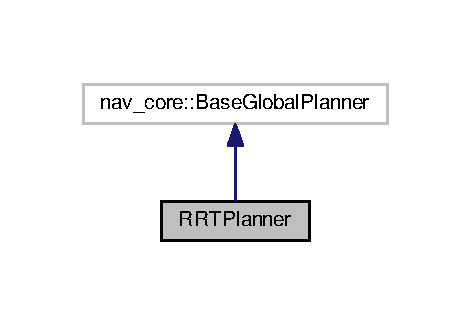
\includegraphics[width=226pt]{classRRTPlanner__coll__graph}
\end{center}
\end{figure}
\subsection*{Public Member Functions}
\begin{DoxyCompactItemize}
\item 
\hyperlink{classRRTPlanner_a1cbf32fc5cc6dd54404f3ffd25abe34c}{R\+R\+T\+Planner} ()\hypertarget{classRRTPlanner_a1cbf32fc5cc6dd54404f3ffd25abe34c}{}\label{classRRTPlanner_a1cbf32fc5cc6dd54404f3ffd25abe34c}

\begin{DoxyCompactList}\small\item\em The default constructor for the \hyperlink{classRRTPlanner}{R\+R\+T\+Planner}. \end{DoxyCompactList}\item 
\hyperlink{classRRTPlanner_a1f5ba162fab96f8efbf87f4b106d8790}{R\+R\+T\+Planner} (std\+::string name, costmap\+\_\+2d\+::\+Costmap2\+D\+R\+OS $\ast$costmap\+Ros)
\begin{DoxyCompactList}\small\item\em Constructor for the \hyperlink{classRRTPlanner}{R\+R\+T\+Planner}. \end{DoxyCompactList}\item 
void \hyperlink{classRRTPlanner_af5b3c48c51620d4e94f8a634589e86fb}{initialize} (std\+::string name, costmap\+\_\+2d\+::\+Costmap2\+D\+R\+OS $\ast$costmap\+Ros)
\begin{DoxyCompactList}\small\item\em Initializes the planner. \end{DoxyCompactList}\item 
bool \hyperlink{classRRTPlanner_ab9abaa15f3deee70dfda2de38f1a6e49}{make\+Plan} (const geometry\+\_\+msgs\+::\+Pose\+Stamped \&start, const geometry\+\_\+msgs\+::\+Pose\+Stamped \&goal, std\+::vector$<$ geometry\+\_\+msgs\+::\+Pose\+Stamped $>$ \&plan)
\begin{DoxyCompactList}\small\item\em Begins the path planner algorithm to generate a plan. \end{DoxyCompactList}\end{DoxyCompactItemize}


\subsection{Constructor \& Destructor Documentation}
\index{R\+R\+T\+Planner@{R\+R\+T\+Planner}!R\+R\+T\+Planner@{R\+R\+T\+Planner}}
\index{R\+R\+T\+Planner@{R\+R\+T\+Planner}!R\+R\+T\+Planner@{R\+R\+T\+Planner}}
\subsubsection[{\texorpdfstring{R\+R\+T\+Planner(std\+::string name, costmap\+\_\+2d\+::\+Costmap2\+D\+R\+O\+S $\ast$costmap\+Ros)}{RRTPlanner(std::string name, costmap_2d::Costmap2DROS *costmapRos)}}]{\setlength{\rightskip}{0pt plus 5cm}R\+R\+T\+Planner\+::\+R\+R\+T\+Planner (
\begin{DoxyParamCaption}
\item[{std\+::string}]{name, }
\item[{costmap\+\_\+2d\+::\+Costmap2\+D\+R\+OS $\ast$}]{costmap\+Ros}
\end{DoxyParamCaption}
)}\hypertarget{classRRTPlanner_a1f5ba162fab96f8efbf87f4b106d8790}{}\label{classRRTPlanner_a1f5ba162fab96f8efbf87f4b106d8790}


Constructor for the \hyperlink{classRRTPlanner}{R\+R\+T\+Planner}. 


\begin{DoxyParams}{Parameters}
{\em name} & The name of the planner node \\
\hline
{\em costmap\+Ros} & The costmap to be used in path planning \\
\hline
\end{DoxyParams}


\subsection{Member Function Documentation}
\index{R\+R\+T\+Planner@{R\+R\+T\+Planner}!initialize@{initialize}}
\index{initialize@{initialize}!R\+R\+T\+Planner@{R\+R\+T\+Planner}}
\subsubsection[{\texorpdfstring{initialize(std\+::string name, costmap\+\_\+2d\+::\+Costmap2\+D\+R\+O\+S $\ast$costmap\+Ros)}{initialize(std::string name, costmap_2d::Costmap2DROS *costmapRos)}}]{\setlength{\rightskip}{0pt plus 5cm}void R\+R\+T\+Planner\+::initialize (
\begin{DoxyParamCaption}
\item[{std\+::string}]{name, }
\item[{costmap\+\_\+2d\+::\+Costmap2\+D\+R\+OS $\ast$}]{costmap\+Ros}
\end{DoxyParamCaption}
)}\hypertarget{classRRTPlanner_af5b3c48c51620d4e94f8a634589e86fb}{}\label{classRRTPlanner_af5b3c48c51620d4e94f8a634589e86fb}


Initializes the planner. 


\begin{DoxyParams}{Parameters}
{\em name} & The name of the planner node \\
\hline
{\em costmap\+Ros} & The costmap to be used in path planning \\
\hline
\end{DoxyParams}
\index{R\+R\+T\+Planner@{R\+R\+T\+Planner}!make\+Plan@{make\+Plan}}
\index{make\+Plan@{make\+Plan}!R\+R\+T\+Planner@{R\+R\+T\+Planner}}
\subsubsection[{\texorpdfstring{make\+Plan(const geometry\+\_\+msgs\+::\+Pose\+Stamped \&start, const geometry\+\_\+msgs\+::\+Pose\+Stamped \&goal, std\+::vector$<$ geometry\+\_\+msgs\+::\+Pose\+Stamped $>$ \&plan)}{makePlan(const geometry_msgs::PoseStamped &start, const geometry_msgs::PoseStamped &goal, std::vector< geometry_msgs::PoseStamped > &plan)}}]{\setlength{\rightskip}{0pt plus 5cm}bool R\+R\+T\+Planner\+::make\+Plan (
\begin{DoxyParamCaption}
\item[{const geometry\+\_\+msgs\+::\+Pose\+Stamped \&}]{start, }
\item[{const geometry\+\_\+msgs\+::\+Pose\+Stamped \&}]{goal, }
\item[{std\+::vector$<$ geometry\+\_\+msgs\+::\+Pose\+Stamped $>$ \&}]{plan}
\end{DoxyParamCaption}
)}\hypertarget{classRRTPlanner_ab9abaa15f3deee70dfda2de38f1a6e49}{}\label{classRRTPlanner_ab9abaa15f3deee70dfda2de38f1a6e49}


Begins the path planner algorithm to generate a plan. 


\begin{DoxyParams}{Parameters}
{\em start} & The start pose of the robot \\
\hline
{\em goal} & The goal pose of the robot \\
\hline
\end{DoxyParams}
\begin{DoxyReturn}{Returns}
0 if no plan was found, and 1 if a plan was generated 
\end{DoxyReturn}


The documentation for this class was generated from the following files\+:\begin{DoxyCompactItemize}
\item 
/home/sammie/catkin\+\_\+ws/src/envi\+\_\+nav/include/\hyperlink{RRTPlanner_8h}{R\+R\+T\+Planner.\+h}\item 
/home/sammie/catkin\+\_\+ws/src/envi\+\_\+nav/src/\hyperlink{RRTPlanner_8cpp}{R\+R\+T\+Planner.\+cpp}\end{DoxyCompactItemize}

\hypertarget{classRRTPlannerHelper}{}\section{R\+R\+T\+Planner\+Helper Class Reference}
\label{classRRTPlannerHelper}\index{R\+R\+T\+Planner\+Helper@{R\+R\+T\+Planner\+Helper}}
\subsection*{Classes}
\begin{DoxyCompactItemize}
\item 
struct \hyperlink{structRRTPlannerHelper_1_1qTree}{q\+Tree}
\begin{DoxyCompactList}\small\item\em Structure that holds the data related to each node in the tree. \end{DoxyCompactList}\end{DoxyCompactItemize}
\subsection*{Public Member Functions}
\begin{DoxyCompactItemize}
\item 
\hyperlink{classRRTPlannerHelper_af99e3fe000e73de8256f59d89c592e96}{R\+R\+T\+Planner\+Helper} (costmap\+\_\+2d\+::\+Costmap2D $\ast$costmap, int mapX, int mapY, float resolution, float originX, float originY, const geometry\+\_\+msgs\+::\+Pose\+Stamped goal, const geometry\+\_\+msgs\+::\+Pose\+Stamped start)
\begin{DoxyCompactList}\small\item\em Constructor for the class. \end{DoxyCompactList}\item 
geometry\+\_\+msgs\+::\+Pose\+Stamped \hyperlink{classRRTPlannerHelper_aae3ca3af6424a1014af42db124e5cd4a}{rand\+\_\+config} ()
\begin{DoxyCompactList}\small\item\em Gets a random X and Y coordinate to create a new node in the tree. \end{DoxyCompactList}\item 
int \hyperlink{classRRTPlannerHelper_a939aa6f8a7eeb2142cc554a8790614bd}{nearest\+\_\+vertex} (geometry\+\_\+msgs\+::\+Pose\+Stamped q\+Rand, std\+::vector$<$ \hyperlink{structRRTPlannerHelper_1_1qTree}{q\+Tree} $>$ tree\+Graph)
\begin{DoxyCompactList}\small\item\em Gets the nearest node in the tree. \end{DoxyCompactList}\item 
bool \hyperlink{classRRTPlannerHelper_a4beec66805ee1ddd248b34054d62e3eb}{path\+\_\+safe} (geometry\+\_\+msgs\+::\+Pose\+Stamped q\+Rand, int i\+Near, std\+::vector$<$ \hyperlink{structRRTPlannerHelper_1_1qTree}{q\+Tree} $>$ tree\+Graph)
\begin{DoxyCompactList}\small\item\em Checks that the path between the two nodes is safe. \end{DoxyCompactList}\item 
bool \hyperlink{classRRTPlannerHelper_aebf2950bb391ab168ac677f56c851575}{check\+\_\+goal} (geometry\+\_\+msgs\+::\+Pose\+Stamped q\+New)
\begin{DoxyCompactList}\small\item\em Checks that the path between the newly added node and the goal is safe. \end{DoxyCompactList}\item 
std\+::vector$<$ geometry\+\_\+msgs\+::\+Pose\+Stamped $>$ \hyperlink{classRRTPlannerHelper_a76d080da45ea6b5d7163dfc7bce3daf7}{build\+\_\+plan} (std\+::vector$<$ \hyperlink{structRRTPlannerHelper_1_1qTree}{q\+Tree} $>$ tree\+Graph)
\begin{DoxyCompactList}\small\item\em Builds the planned path from the node tree. \end{DoxyCompactList}\item 
void \hyperlink{classRRTPlannerHelper_afde8ae441b0c245d4ea35546cf3628c8}{rviz\+\_\+map} (double \&x, double \&y)
\begin{DoxyCompactList}\small\item\em Converts the coordinates given from rviz to costmap coordinates. \end{DoxyCompactList}\item 
void \hyperlink{classRRTPlannerHelper_a7616495b1de44739bc8decda8dce3691}{map\+\_\+rviz} (double \&x, double \&y)
\begin{DoxyCompactList}\small\item\em Converts the coordinates from the costmap to rviz coordinates. \end{DoxyCompactList}\end{DoxyCompactItemize}
\subsection*{Public Attributes}
\begin{DoxyCompactItemize}
\item 
std\+::vector$<$ geometry\+\_\+msgs\+::\+Pose\+Stamped $>$ {\bfseries \+\_\+plan}\hypertarget{classRRTPlannerHelper_ac29ee7b115e06233770f5ae0adaabfc4}{}\label{classRRTPlannerHelper_ac29ee7b115e06233770f5ae0adaabfc4}

\item 
geometry\+\_\+msgs\+::\+Pose\+Stamped {\bfseries \+\_\+goal}\hypertarget{classRRTPlannerHelper_a05a168ac5796fa9223fc65e9a34adefd}{}\label{classRRTPlannerHelper_a05a168ac5796fa9223fc65e9a34adefd}

\item 
geometry\+\_\+msgs\+::\+Pose\+Stamped {\bfseries \+\_\+start}\hypertarget{classRRTPlannerHelper_a9ce6ea01d2c7fc50eb1ac295bedcab08}{}\label{classRRTPlannerHelper_a9ce6ea01d2c7fc50eb1ac295bedcab08}

\item 
costmap\+\_\+2d\+::\+Costmap2D $\ast$ {\bfseries \+\_\+costmap}\hypertarget{classRRTPlannerHelper_a8022e8bc3b5d3358cbad20d804045f1f}{}\label{classRRTPlannerHelper_a8022e8bc3b5d3358cbad20d804045f1f}

\item 
float {\bfseries \+\_\+resolution}\hypertarget{classRRTPlannerHelper_a10ec2c02a83af5ee89298a799581e508}{}\label{classRRTPlannerHelper_a10ec2c02a83af5ee89298a799581e508}

\item 
float {\bfseries \+\_\+originX}\hypertarget{classRRTPlannerHelper_a5420ff18107881ea63e902a0d3a74aac}{}\label{classRRTPlannerHelper_a5420ff18107881ea63e902a0d3a74aac}

\item 
float {\bfseries \+\_\+originY}\hypertarget{classRRTPlannerHelper_a08961873e85b14e462ea84c2d39c20ff}{}\label{classRRTPlannerHelper_a08961873e85b14e462ea84c2d39c20ff}

\item 
int {\bfseries \+\_\+map\+SizeX}\hypertarget{classRRTPlannerHelper_a69639eb4295147df9995de9a0727ff27}{}\label{classRRTPlannerHelper_a69639eb4295147df9995de9a0727ff27}

\item 
int {\bfseries \+\_\+map\+SizeY}\hypertarget{classRRTPlannerHelper_a70a60acd18da760aae8f8181c133faa7}{}\label{classRRTPlannerHelper_a70a60acd18da760aae8f8181c133faa7}

\item 
double {\bfseries \+\_\+allowed\+Dist}\hypertarget{classRRTPlannerHelper_a4f305d9c128499eba054960e29f1989d}{}\label{classRRTPlannerHelper_a4f305d9c128499eba054960e29f1989d}

\end{DoxyCompactItemize}


\subsection{Constructor \& Destructor Documentation}
\index{R\+R\+T\+Planner\+Helper@{R\+R\+T\+Planner\+Helper}!R\+R\+T\+Planner\+Helper@{R\+R\+T\+Planner\+Helper}}
\index{R\+R\+T\+Planner\+Helper@{R\+R\+T\+Planner\+Helper}!R\+R\+T\+Planner\+Helper@{R\+R\+T\+Planner\+Helper}}
\subsubsection[{\texorpdfstring{R\+R\+T\+Planner\+Helper(costmap\+\_\+2d\+::\+Costmap2\+D $\ast$costmap, int map\+X, int map\+Y, float resolution, float origin\+X, float origin\+Y, const geometry\+\_\+msgs\+::\+Pose\+Stamped goal, const geometry\+\_\+msgs\+::\+Pose\+Stamped start)}{RRTPlannerHelper(costmap_2d::Costmap2D *costmap, int mapX, int mapY, float resolution, float originX, float originY, const geometry_msgs::PoseStamped goal, const geometry_msgs::PoseStamped start)}}]{\setlength{\rightskip}{0pt plus 5cm}R\+R\+T\+Planner\+Helper\+::\+R\+R\+T\+Planner\+Helper (
\begin{DoxyParamCaption}
\item[{costmap\+\_\+2d\+::\+Costmap2D $\ast$}]{costmap, }
\item[{int}]{mapX, }
\item[{int}]{mapY, }
\item[{float}]{resolution, }
\item[{float}]{originX, }
\item[{float}]{originY, }
\item[{const geometry\+\_\+msgs\+::\+Pose\+Stamped}]{goal, }
\item[{const geometry\+\_\+msgs\+::\+Pose\+Stamped}]{start}
\end{DoxyParamCaption}
)}\hypertarget{classRRTPlannerHelper_af99e3fe000e73de8256f59d89c592e96}{}\label{classRRTPlannerHelper_af99e3fe000e73de8256f59d89c592e96}


Constructor for the class. 


\begin{DoxyParams}{Parameters}
{\em costmap} & The costmap used in path planning \\
\hline
{\em mapX} & The size of the map in x coordinates \\
\hline
{\em mapY} & The size of the map in y coordinates \\
\hline
{\em resolution} & The resolution of the costmap \\
\hline
{\em originX} & The x origin of the costmap \\
\hline
{\em originY} & The y origin of the costmap \\
\hline
{\em goal} & The given goal pose for the robot \\
\hline
{\em start} & The given start pose of the robot \\
\hline
\end{DoxyParams}


\subsection{Member Function Documentation}
\index{R\+R\+T\+Planner\+Helper@{R\+R\+T\+Planner\+Helper}!build\+\_\+plan@{build\+\_\+plan}}
\index{build\+\_\+plan@{build\+\_\+plan}!R\+R\+T\+Planner\+Helper@{R\+R\+T\+Planner\+Helper}}
\subsubsection[{\texorpdfstring{build\+\_\+plan(std\+::vector$<$ q\+Tree $>$ tree\+Graph)}{build_plan(std::vector< qTree > treeGraph)}}]{\setlength{\rightskip}{0pt plus 5cm}std\+::vector$<$ geometry\+\_\+msgs\+::\+Pose\+Stamped $>$ R\+R\+T\+Planner\+Helper\+::build\+\_\+plan (
\begin{DoxyParamCaption}
\item[{std\+::vector$<$ {\bf q\+Tree} $>$}]{tree\+Graph}
\end{DoxyParamCaption}
)}\hypertarget{classRRTPlannerHelper_a76d080da45ea6b5d7163dfc7bce3daf7}{}\label{classRRTPlannerHelper_a76d080da45ea6b5d7163dfc7bce3daf7}


Builds the planned path from the node tree. 


\begin{DoxyParams}{Parameters}
{\em tree\+Graph} & The set of all of the nodes in the tree \\
\hline
\end{DoxyParams}
\begin{DoxyReturn}{Returns}
The global path plan that was generated by the R\+RT algorithm 
\end{DoxyReturn}
\index{R\+R\+T\+Planner\+Helper@{R\+R\+T\+Planner\+Helper}!check\+\_\+goal@{check\+\_\+goal}}
\index{check\+\_\+goal@{check\+\_\+goal}!R\+R\+T\+Planner\+Helper@{R\+R\+T\+Planner\+Helper}}
\subsubsection[{\texorpdfstring{check\+\_\+goal(geometry\+\_\+msgs\+::\+Pose\+Stamped q\+New)}{check_goal(geometry_msgs::PoseStamped qNew)}}]{\setlength{\rightskip}{0pt plus 5cm}bool R\+R\+T\+Planner\+Helper\+::check\+\_\+goal (
\begin{DoxyParamCaption}
\item[{geometry\+\_\+msgs\+::\+Pose\+Stamped}]{q\+New}
\end{DoxyParamCaption}
)}\hypertarget{classRRTPlannerHelper_aebf2950bb391ab168ac677f56c851575}{}\label{classRRTPlannerHelper_aebf2950bb391ab168ac677f56c851575}


Checks that the path between the newly added node and the goal is safe. 


\begin{DoxyParams}{Parameters}
{\em q\+New} & The new configuration added to the tree \\
\hline
\end{DoxyParams}
\begin{DoxyReturn}{Returns}
0 if path is blocked, and 1 if the path is clear 
\end{DoxyReturn}
\index{R\+R\+T\+Planner\+Helper@{R\+R\+T\+Planner\+Helper}!map\+\_\+rviz@{map\+\_\+rviz}}
\index{map\+\_\+rviz@{map\+\_\+rviz}!R\+R\+T\+Planner\+Helper@{R\+R\+T\+Planner\+Helper}}
\subsubsection[{\texorpdfstring{map\+\_\+rviz(double \&x, double \&y)}{map_rviz(double &x, double &y)}}]{\setlength{\rightskip}{0pt plus 5cm}void R\+R\+T\+Planner\+Helper\+::map\+\_\+rviz (
\begin{DoxyParamCaption}
\item[{double \&}]{x, }
\item[{double \&}]{y}
\end{DoxyParamCaption}
)}\hypertarget{classRRTPlannerHelper_a7616495b1de44739bc8decda8dce3691}{}\label{classRRTPlannerHelper_a7616495b1de44739bc8decda8dce3691}


Converts the coordinates from the costmap to rviz coordinates. 


\begin{DoxyParams}{Parameters}
{\em x} & The x component of the coordinate, this gets updated \\
\hline
{\em y} & The y component of the coordinate, this gets updated \\
\hline
\end{DoxyParams}
\index{R\+R\+T\+Planner\+Helper@{R\+R\+T\+Planner\+Helper}!nearest\+\_\+vertex@{nearest\+\_\+vertex}}
\index{nearest\+\_\+vertex@{nearest\+\_\+vertex}!R\+R\+T\+Planner\+Helper@{R\+R\+T\+Planner\+Helper}}
\subsubsection[{\texorpdfstring{nearest\+\_\+vertex(geometry\+\_\+msgs\+::\+Pose\+Stamped q\+Rand, std\+::vector$<$ q\+Tree $>$ tree\+Graph)}{nearest_vertex(geometry_msgs::PoseStamped qRand, std::vector< qTree > treeGraph)}}]{\setlength{\rightskip}{0pt plus 5cm}int R\+R\+T\+Planner\+Helper\+::nearest\+\_\+vertex (
\begin{DoxyParamCaption}
\item[{geometry\+\_\+msgs\+::\+Pose\+Stamped}]{q\+Rand, }
\item[{std\+::vector$<$ {\bf q\+Tree} $>$}]{tree\+Graph}
\end{DoxyParamCaption}
)}\hypertarget{classRRTPlannerHelper_a939aa6f8a7eeb2142cc554a8790614bd}{}\label{classRRTPlannerHelper_a939aa6f8a7eeb2142cc554a8790614bd}


Gets the nearest node in the tree. 


\begin{DoxyParams}{Parameters}
{\em q\+Rand} & The randomly generated pose for the robot \\
\hline
{\em tree\+Graph} & The set of all of the nodes if the tree \\
\hline
\end{DoxyParams}
\begin{DoxyReturn}{Returns}
The index of the nearest vertex in the tree 
\end{DoxyReturn}
\index{R\+R\+T\+Planner\+Helper@{R\+R\+T\+Planner\+Helper}!path\+\_\+safe@{path\+\_\+safe}}
\index{path\+\_\+safe@{path\+\_\+safe}!R\+R\+T\+Planner\+Helper@{R\+R\+T\+Planner\+Helper}}
\subsubsection[{\texorpdfstring{path\+\_\+safe(geometry\+\_\+msgs\+::\+Pose\+Stamped q\+Rand, int i\+Near, std\+::vector$<$ q\+Tree $>$ tree\+Graph)}{path_safe(geometry_msgs::PoseStamped qRand, int iNear, std::vector< qTree > treeGraph)}}]{\setlength{\rightskip}{0pt plus 5cm}bool R\+R\+T\+Planner\+Helper\+::path\+\_\+safe (
\begin{DoxyParamCaption}
\item[{geometry\+\_\+msgs\+::\+Pose\+Stamped}]{q\+Rand, }
\item[{int}]{i\+Near, }
\item[{std\+::vector$<$ {\bf q\+Tree} $>$}]{tree\+Graph}
\end{DoxyParamCaption}
)}\hypertarget{classRRTPlannerHelper_a4beec66805ee1ddd248b34054d62e3eb}{}\label{classRRTPlannerHelper_a4beec66805ee1ddd248b34054d62e3eb}


Checks that the path between the two nodes is safe. 


\begin{DoxyParams}{Parameters}
{\em q\+Rand} & The new random configuration \\
\hline
{\em i\+Near} & The index of the nearest node in the tree \\
\hline
{\em tree\+Graph} & The set of all of the nodes in the tree \\
\hline
\end{DoxyParams}
\begin{DoxyReturn}{Returns}
0 if the path is blocked, and 1 if the path is clear 
\end{DoxyReturn}
\index{R\+R\+T\+Planner\+Helper@{R\+R\+T\+Planner\+Helper}!rand\+\_\+config@{rand\+\_\+config}}
\index{rand\+\_\+config@{rand\+\_\+config}!R\+R\+T\+Planner\+Helper@{R\+R\+T\+Planner\+Helper}}
\subsubsection[{\texorpdfstring{rand\+\_\+config()}{rand_config()}}]{\setlength{\rightskip}{0pt plus 5cm}geometry\+\_\+msgs\+::\+Pose\+Stamped R\+R\+T\+Planner\+Helper\+::rand\+\_\+config (
\begin{DoxyParamCaption}
{}
\end{DoxyParamCaption}
)}\hypertarget{classRRTPlannerHelper_aae3ca3af6424a1014af42db124e5cd4a}{}\label{classRRTPlannerHelper_aae3ca3af6424a1014af42db124e5cd4a}


Gets a random X and Y coordinate to create a new node in the tree. 

\begin{DoxyReturn}{Returns}
A random configuration that lies in the costmap 
\end{DoxyReturn}
\index{R\+R\+T\+Planner\+Helper@{R\+R\+T\+Planner\+Helper}!rviz\+\_\+map@{rviz\+\_\+map}}
\index{rviz\+\_\+map@{rviz\+\_\+map}!R\+R\+T\+Planner\+Helper@{R\+R\+T\+Planner\+Helper}}
\subsubsection[{\texorpdfstring{rviz\+\_\+map(double \&x, double \&y)}{rviz_map(double &x, double &y)}}]{\setlength{\rightskip}{0pt plus 5cm}void R\+R\+T\+Planner\+Helper\+::rviz\+\_\+map (
\begin{DoxyParamCaption}
\item[{double \&}]{x, }
\item[{double \&}]{y}
\end{DoxyParamCaption}
)}\hypertarget{classRRTPlannerHelper_afde8ae441b0c245d4ea35546cf3628c8}{}\label{classRRTPlannerHelper_afde8ae441b0c245d4ea35546cf3628c8}


Converts the coordinates given from rviz to costmap coordinates. 


\begin{DoxyParams}{Parameters}
{\em x} & The x component of the coordinate, this gets updated \\
\hline
{\em y} & The y component of the coordinate, this gets updated \\
\hline
\end{DoxyParams}


The documentation for this class was generated from the following files\+:\begin{DoxyCompactItemize}
\item 
/home/sammie/catkin\+\_\+ws/src/envi\+\_\+nav/include/\hyperlink{RRTPlannerHelper_8h}{R\+R\+T\+Planner\+Helper.\+h}\item 
/home/sammie/catkin\+\_\+ws/src/envi\+\_\+nav/src/\hyperlink{RRTPlannerHelper_8cpp}{R\+R\+T\+Planner\+Helper.\+cpp}\end{DoxyCompactItemize}

\hypertarget{classRRTPlannerTester}{}\section{R\+R\+T\+Planner\+Tester Class Reference}
\label{classRRTPlannerTester}\index{R\+R\+T\+Planner\+Tester@{R\+R\+T\+Planner\+Tester}}
\subsection*{Public Member Functions}
\begin{DoxyCompactItemize}
\item 
\hyperlink{classRRTPlannerHelper}{R\+R\+T\+Planner\+Helper} {\bfseries get\+Helper} ()\hypertarget{classRRTPlannerTester_af2bf60de841e92af66a7440831916886}{}\label{classRRTPlannerTester_af2bf60de841e92af66a7440831916886}

\end{DoxyCompactItemize}
\subsection*{Public Attributes}
\begin{DoxyCompactItemize}
\item 
costmap\+\_\+2d\+::\+Costmap2\+D\+R\+OS $\ast$ {\bfseries costmap\+Ros}\hypertarget{classRRTPlannerTester_af23925ac3623b7f6e831e519e861091a}{}\label{classRRTPlannerTester_af23925ac3623b7f6e831e519e861091a}

\end{DoxyCompactItemize}


The documentation for this class was generated from the following file\+:\begin{DoxyCompactItemize}
\item 
/home/sammie/catkin\+\_\+ws/src/envi\+\_\+nav/test/\hyperlink{EnviNavTests_8cpp}{Envi\+Nav\+Tests.\+cpp}\end{DoxyCompactItemize}

\chapter{File Documentation}
\hypertarget{MapBuild_8h}{}\section{/home/sammie/catkin\+\_\+ws/src/envi\+\_\+nav/include/\+Map\+Build.h File Reference}
\label{MapBuild_8h}\index{/home/sammie/catkin\+\_\+ws/src/envi\+\_\+nav/include/\+Map\+Build.\+h@{/home/sammie/catkin\+\_\+ws/src/envi\+\_\+nav/include/\+Map\+Build.\+h}}


Saves the map generated by the navigation demo.  


{\ttfamily \#include $<$ros/ros.\+h$>$}\\*
{\ttfamily \#include $<$sstream$>$}\\*
{\ttfamily \#include $<$string$>$}\\*
Include dependency graph for Map\+Build.\+h\+:\nopagebreak
\begin{figure}[H]
\begin{center}
\leavevmode
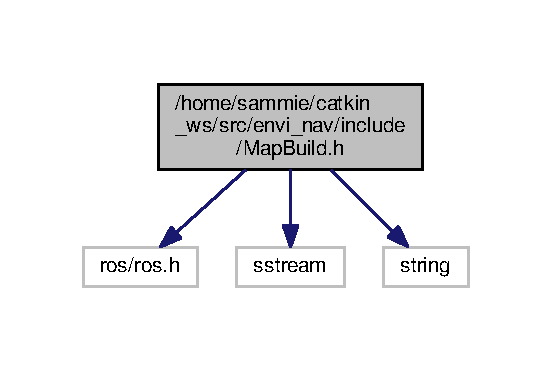
\includegraphics[width=265pt]{MapBuild_8h__incl}
\end{center}
\end{figure}
This graph shows which files directly or indirectly include this file\+:\nopagebreak
\begin{figure}[H]
\begin{center}
\leavevmode
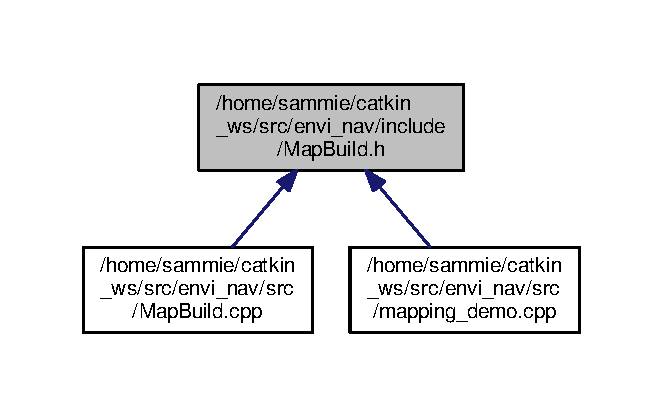
\includegraphics[width=318pt]{MapBuild_8h__dep__incl}
\end{center}
\end{figure}
\subsection*{Classes}
\begin{DoxyCompactItemize}
\item 
class \hyperlink{classMapBuild}{Map\+Build}
\end{DoxyCompactItemize}


\subsection{Detailed Description}
Saves the map generated by the navigation demo. 

\begin{DoxyAuthor}{Author}
Samantha Johnson 
\end{DoxyAuthor}
\begin{DoxyDate}{Date}
December 15, 2017  B\+SD 3-\/\+Clause License 
\end{DoxyDate}
\begin{DoxyCopyright}{Copyright}
(c) 2017, Samantha Johnson All rights reserved.
\end{DoxyCopyright}
Redistribution and use in source and binary forms, with or without modification, are permitted provided that the following conditions are met\+:

Redistributions of source code must retain the above copyright notice, this list of conditions and the following disclaimer.

Redistributions in binary form must reproduce the above copyright notice, this list of conditions and the following disclaimer in the documentation and/or other materials provided with the distribution.

Neither the name of the copyright holder nor the names of its contributors may be used to endorse or promote products derived from this software without specific prior written permission.

T\+H\+IS S\+O\+F\+T\+W\+A\+RE IS P\+R\+O\+V\+I\+D\+ED BY T\+HE C\+O\+P\+Y\+R\+I\+G\+HT H\+O\+L\+D\+E\+RS A\+ND C\+O\+N\+T\+R\+I\+B\+U\+T\+O\+RS \char`\"{}\+A\+S I\+S\char`\"{} A\+ND A\+NY E\+X\+P\+R\+E\+SS OR I\+M\+P\+L\+I\+ED W\+A\+R\+R\+A\+N\+T\+I\+ES, I\+N\+C\+L\+U\+D\+I\+NG, B\+UT N\+OT L\+I\+M\+I\+T\+ED TO, T\+HE I\+M\+P\+L\+I\+ED W\+A\+R\+R\+A\+N\+T\+I\+ES OF M\+E\+R\+C\+H\+A\+N\+T\+A\+B\+I\+L\+I\+TY A\+ND F\+I\+T\+N\+E\+SS F\+OR A P\+A\+R\+T\+I\+C\+U\+L\+AR P\+U\+R\+P\+O\+SE A\+RE D\+I\+S\+C\+L\+A\+I\+M\+ED. IN NO E\+V\+E\+NT S\+H\+A\+LL T\+HE C\+O\+P\+Y\+R\+I\+G\+HT H\+O\+L\+D\+ER OR C\+O\+N\+T\+R\+I\+B\+U\+T\+O\+RS BE L\+I\+A\+B\+LE F\+OR A\+NY D\+I\+R\+E\+CT, I\+N\+D\+I\+R\+E\+CT, I\+N\+C\+I\+D\+E\+N\+T\+AL, S\+P\+E\+C\+I\+AL, E\+X\+E\+M\+P\+L\+A\+RY, OR C\+O\+N\+S\+E\+Q\+U\+E\+N\+T\+I\+AL D\+A\+M\+A\+G\+ES (I\+N\+C\+L\+U\+D\+I\+NG, B\+UT N\+OT L\+I\+M\+I\+T\+ED TO, P\+R\+O\+C\+U\+R\+E\+M\+E\+NT OF S\+U\+B\+S\+T\+I\+T\+U\+TE G\+O\+O\+DS OR S\+E\+R\+V\+I\+C\+ES; L\+O\+SS OF U\+SE, D\+A\+TA, OR P\+R\+O\+F\+I\+TS; OR B\+U\+S\+I\+N\+E\+SS I\+N\+T\+E\+R\+R\+U\+P\+T\+I\+ON) H\+O\+W\+E\+V\+ER C\+A\+U\+S\+ED A\+ND ON A\+NY T\+H\+E\+O\+RY OF L\+I\+A\+B\+I\+L\+I\+TY, W\+H\+E\+T\+H\+ER IN C\+O\+N\+T\+R\+A\+CT, S\+T\+R\+I\+CT L\+I\+A\+B\+I\+L\+I\+TY, OR T\+O\+RT (I\+N\+C\+L\+U\+D\+I\+NG N\+E\+G\+L\+I\+G\+E\+N\+CE OR O\+T\+H\+E\+R\+W\+I\+SE) A\+R\+I\+S\+I\+NG IN A\+NY W\+AY O\+UT OF T\+HE U\+SE OF T\+H\+IS S\+O\+F\+T\+W\+A\+RE, E\+V\+EN IF A\+D\+V\+I\+S\+ED OF T\+HE P\+O\+S\+S\+I\+B\+I\+L\+I\+TY OF S\+U\+CH D\+A\+M\+A\+GE.

Allows the user to save the map being built in the navigation demo by typing a simple command. 
\hypertarget{RRTPlanner_8h}{}\section{/home/sammie/catkin\+\_\+ws/src/envi\+\_\+nav/include/\+R\+R\+T\+Planner.h File Reference}
\label{RRTPlanner_8h}\index{/home/sammie/catkin\+\_\+ws/src/envi\+\_\+nav/include/\+R\+R\+T\+Planner.\+h@{/home/sammie/catkin\+\_\+ws/src/envi\+\_\+nav/include/\+R\+R\+T\+Planner.\+h}}


Global path planner implementing the R\+RT algorithm.  


{\ttfamily \#include $<$ros/ros.\+h$>$}\\*
{\ttfamily \#include $<$costmap\+\_\+2d/costmap\+\_\+2d\+\_\+ros.\+h$>$}\\*
{\ttfamily \#include $<$costmap\+\_\+2d/costmap\+\_\+2d.\+h$>$}\\*
{\ttfamily \#include $<$nav\+\_\+core/base\+\_\+global\+\_\+planner.\+h$>$}\\*
{\ttfamily \#include $<$geometry\+\_\+msgs/\+Pose\+Stamped.\+h$>$}\\*
{\ttfamily \#include $<$pluginlib/class\+\_\+list\+\_\+macros.\+h$>$}\\*
{\ttfamily \#include $<$algorithm$>$}\\*
{\ttfamily \#include $<$vector$>$}\\*
{\ttfamily \#include $<$string$>$}\\*
Include dependency graph for R\+R\+T\+Planner.\+h\+:\nopagebreak
\begin{figure}[H]
\begin{center}
\leavevmode
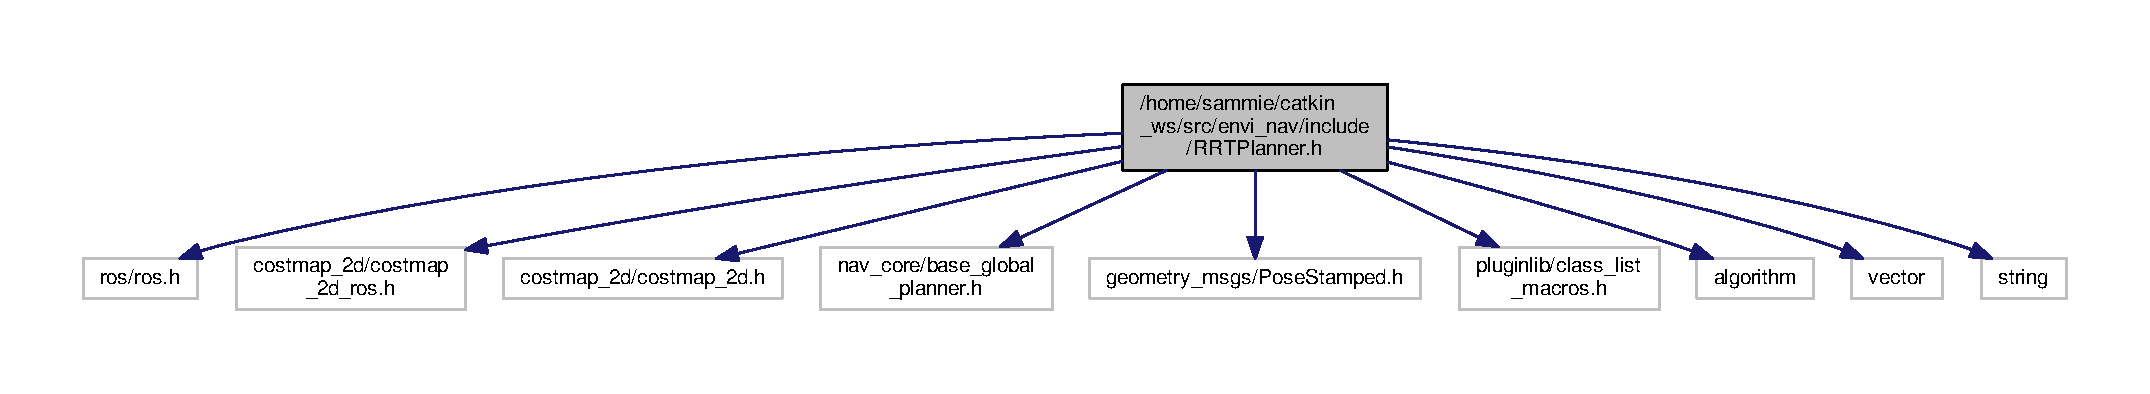
\includegraphics[width=350pt]{RRTPlanner_8h__incl}
\end{center}
\end{figure}
This graph shows which files directly or indirectly include this file\+:\nopagebreak
\begin{figure}[H]
\begin{center}
\leavevmode
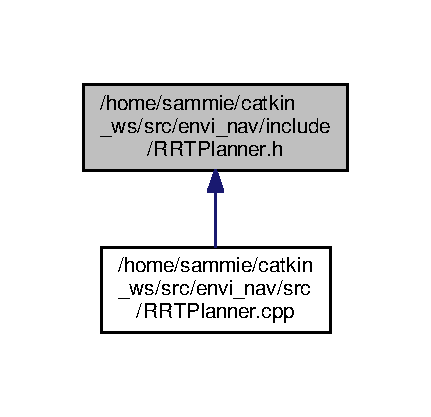
\includegraphics[width=207pt]{RRTPlanner_8h__dep__incl}
\end{center}
\end{figure}
\subsection*{Classes}
\begin{DoxyCompactItemize}
\item 
class \hyperlink{classRRTPlanner}{R\+R\+T\+Planner}
\end{DoxyCompactItemize}


\subsection{Detailed Description}
Global path planner implementing the R\+RT algorithm. 

\begin{DoxyAuthor}{Author}
Samantha Johnson 
\end{DoxyAuthor}
\begin{DoxyDate}{Date}
December 15, 2017  B\+SD 3-\/\+Clause License 
\end{DoxyDate}
\begin{DoxyCopyright}{Copyright}
(c) 2017, Samantha Johnson All rights reserved.
\end{DoxyCopyright}
Redistribution and use in source and binary forms, with or without modification, are permitted provided that the following conditions are met\+:

Redistributions of source code must retain the above copyright notice, this list of conditions and the following disclaimer.

Redistributions in binary form must reproduce the above copyright notice, this list of conditions and the following disclaimer in the documentation and/or other materials provided with the distribution.

Neither the name of the copyright holder nor the names of its contributors may be used to endorse or promote products derived from this software without specific prior written permission.

T\+H\+IS S\+O\+F\+T\+W\+A\+RE IS P\+R\+O\+V\+I\+D\+ED BY T\+HE C\+O\+P\+Y\+R\+I\+G\+HT H\+O\+L\+D\+E\+RS A\+ND C\+O\+N\+T\+R\+I\+B\+U\+T\+O\+RS \char`\"{}\+A\+S I\+S\char`\"{} A\+ND A\+NY E\+X\+P\+R\+E\+SS OR I\+M\+P\+L\+I\+ED W\+A\+R\+R\+A\+N\+T\+I\+ES, I\+N\+C\+L\+U\+D\+I\+NG, B\+UT N\+OT L\+I\+M\+I\+T\+ED TO, T\+HE I\+M\+P\+L\+I\+ED W\+A\+R\+R\+A\+N\+T\+I\+ES OF M\+E\+R\+C\+H\+A\+N\+T\+A\+B\+I\+L\+I\+TY A\+ND F\+I\+T\+N\+E\+SS F\+OR A P\+A\+R\+T\+I\+C\+U\+L\+AR P\+U\+R\+P\+O\+SE A\+RE D\+I\+S\+C\+L\+A\+I\+M\+ED. IN NO E\+V\+E\+NT S\+H\+A\+LL T\+HE C\+O\+P\+Y\+R\+I\+G\+HT H\+O\+L\+D\+ER OR C\+O\+N\+T\+R\+I\+B\+U\+T\+O\+RS BE L\+I\+A\+B\+LE F\+OR A\+NY D\+I\+R\+E\+CT, I\+N\+D\+I\+R\+E\+CT, I\+N\+C\+I\+D\+E\+N\+T\+AL, S\+P\+E\+C\+I\+AL, E\+X\+E\+M\+P\+L\+A\+RY, OR C\+O\+N\+S\+E\+Q\+U\+E\+N\+T\+I\+AL D\+A\+M\+A\+G\+ES (I\+N\+C\+L\+U\+D\+I\+NG, B\+UT N\+OT L\+I\+M\+I\+T\+ED TO, P\+R\+O\+C\+U\+R\+E\+M\+E\+NT OF S\+U\+B\+S\+T\+I\+T\+U\+TE G\+O\+O\+DS OR S\+E\+R\+V\+I\+C\+ES; L\+O\+SS OF U\+SE, D\+A\+TA, OR P\+R\+O\+F\+I\+TS; OR B\+U\+S\+I\+N\+E\+SS I\+N\+T\+E\+R\+R\+U\+P\+T\+I\+ON) H\+O\+W\+E\+V\+ER C\+A\+U\+S\+ED A\+ND ON A\+NY T\+H\+E\+O\+RY OF L\+I\+A\+B\+I\+L\+I\+TY, W\+H\+E\+T\+H\+ER IN C\+O\+N\+T\+R\+A\+CT, S\+T\+R\+I\+CT L\+I\+A\+B\+I\+L\+I\+TY, OR T\+O\+RT (I\+N\+C\+L\+U\+D\+I\+NG N\+E\+G\+L\+I\+G\+E\+N\+CE OR O\+T\+H\+E\+R\+W\+I\+SE) A\+R\+I\+S\+I\+NG IN A\+NY W\+AY O\+UT OF T\+HE U\+SE OF T\+H\+IS S\+O\+F\+T\+W\+A\+RE, E\+V\+EN IF A\+D\+V\+I\+S\+ED OF T\+HE P\+O\+S\+S\+I\+B\+I\+L\+I\+TY OF S\+U\+CH D\+A\+M\+A\+GE.

This plugin was created to interface with the nav\+\_\+core/base\+\_\+global\+\_\+planner framework and replace the default global planner used in the navigation stack. This plugin uses an R\+RT algorithm which generates a path by creating a tree full of random nodes that are connected to their nearest node neighbor if the path is clear. Once the goal is reached by the tree, the planner returns a path which is a connection of the nodes in the tree that traverse from start to goal. 
\hypertarget{RRTPlannerHelper_8h}{}\section{/home/sammie/catkin\+\_\+ws/src/envi\+\_\+nav/include/\+R\+R\+T\+Planner\+Helper.h File Reference}
\label{RRTPlannerHelper_8h}\index{/home/sammie/catkin\+\_\+ws/src/envi\+\_\+nav/include/\+R\+R\+T\+Planner\+Helper.\+h@{/home/sammie/catkin\+\_\+ws/src/envi\+\_\+nav/include/\+R\+R\+T\+Planner\+Helper.\+h}}


Global path planner implementing the R\+RT algorithm.  


{\ttfamily \#include $<$ros/ros.\+h$>$}\\*
{\ttfamily \#include $<$costmap\+\_\+2d/costmap\+\_\+2d\+\_\+ros.\+h$>$}\\*
{\ttfamily \#include $<$costmap\+\_\+2d/costmap\+\_\+2d.\+h$>$}\\*
{\ttfamily \#include $<$nav\+\_\+core/base\+\_\+global\+\_\+planner.\+h$>$}\\*
{\ttfamily \#include $<$geometry\+\_\+msgs/\+Pose\+Stamped.\+h$>$}\\*
{\ttfamily \#include $<$vector$>$}\\*
Include dependency graph for R\+R\+T\+Planner\+Helper.\+h\+:\nopagebreak
\begin{figure}[H]
\begin{center}
\leavevmode
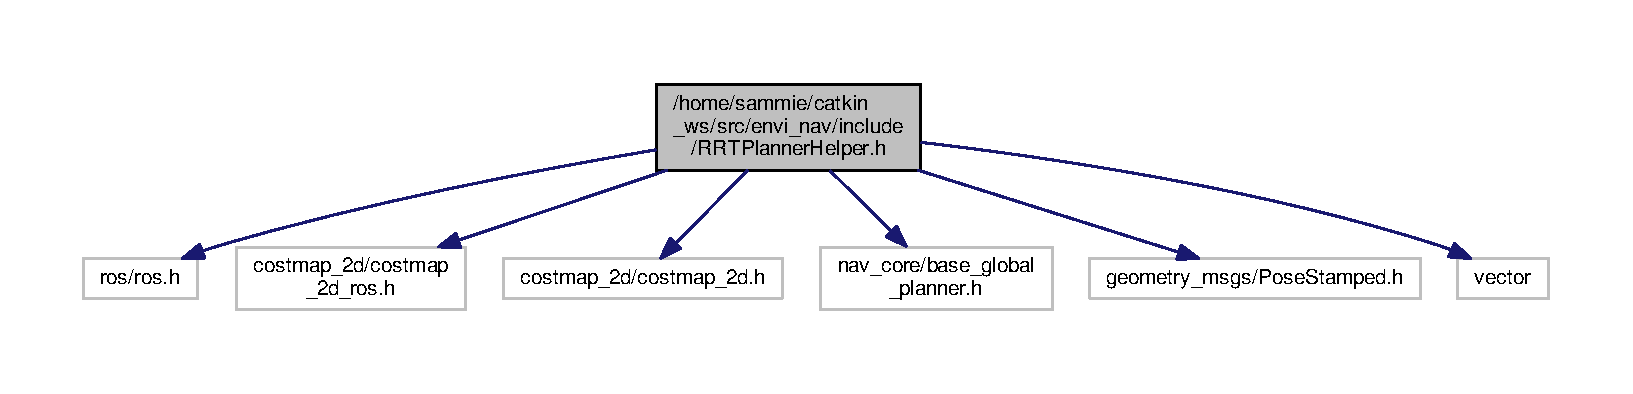
\includegraphics[width=350pt]{RRTPlannerHelper_8h__incl}
\end{center}
\end{figure}
This graph shows which files directly or indirectly include this file\+:\nopagebreak
\begin{figure}[H]
\begin{center}
\leavevmode
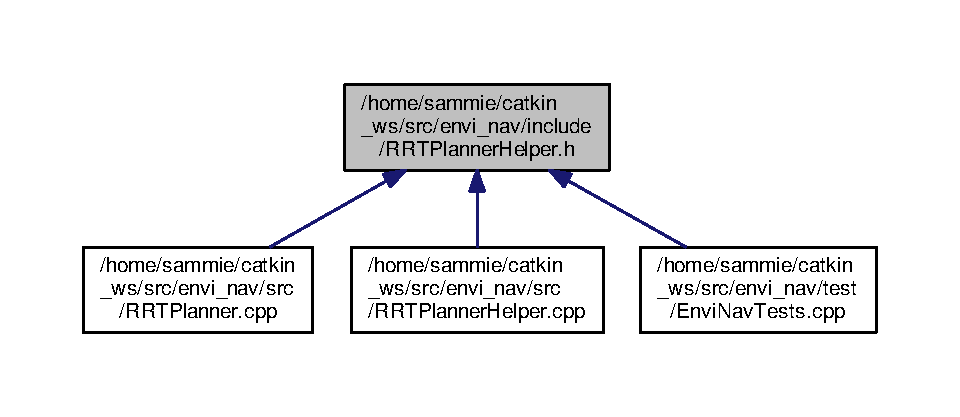
\includegraphics[width=350pt]{RRTPlannerHelper_8h__dep__incl}
\end{center}
\end{figure}
\subsection*{Classes}
\begin{DoxyCompactItemize}
\item 
class \hyperlink{classRRTPlannerHelper}{R\+R\+T\+Planner\+Helper}
\item 
struct \hyperlink{structRRTPlannerHelper_1_1qTree}{R\+R\+T\+Planner\+Helper\+::q\+Tree}
\begin{DoxyCompactList}\small\item\em Structure that holds the data related to each node in the tree. \end{DoxyCompactList}\end{DoxyCompactItemize}


\subsection{Detailed Description}
Global path planner implementing the R\+RT algorithm. 

\begin{DoxyAuthor}{Author}
Samantha Johnson 
\end{DoxyAuthor}
\begin{DoxyDate}{Date}
December 15, 2017  B\+SD 3-\/\+Clause License 
\end{DoxyDate}
\begin{DoxyCopyright}{Copyright}
(c) 2017, Samantha Johnson All rights reserved.
\end{DoxyCopyright}
Redistribution and use in source and binary forms, with or without modification, are permitted provided that the following conditions are met\+:

Redistributions of source code must retain the above copyright notice, this list of conditions and the following disclaimer.

Redistributions in binary form must reproduce the above copyright notice, this list of conditions and the following disclaimer in the documentation and/or other materials provided with the distribution.

Neither the name of the copyright holder nor the names of its contributors may be used to endorse or promote products derived from this software without specific prior written permission.

T\+H\+IS S\+O\+F\+T\+W\+A\+RE IS P\+R\+O\+V\+I\+D\+ED BY T\+HE C\+O\+P\+Y\+R\+I\+G\+HT H\+O\+L\+D\+E\+RS A\+ND C\+O\+N\+T\+R\+I\+B\+U\+T\+O\+RS \char`\"{}\+A\+S I\+S\char`\"{} A\+ND A\+NY E\+X\+P\+R\+E\+SS OR I\+M\+P\+L\+I\+ED W\+A\+R\+R\+A\+N\+T\+I\+ES, I\+N\+C\+L\+U\+D\+I\+NG, B\+UT N\+OT L\+I\+M\+I\+T\+ED TO, T\+HE I\+M\+P\+L\+I\+ED W\+A\+R\+R\+A\+N\+T\+I\+ES OF M\+E\+R\+C\+H\+A\+N\+T\+A\+B\+I\+L\+I\+TY A\+ND F\+I\+T\+N\+E\+SS F\+OR A P\+A\+R\+T\+I\+C\+U\+L\+AR P\+U\+R\+P\+O\+SE A\+RE D\+I\+S\+C\+L\+A\+I\+M\+ED. IN NO E\+V\+E\+NT S\+H\+A\+LL T\+HE C\+O\+P\+Y\+R\+I\+G\+HT H\+O\+L\+D\+ER OR C\+O\+N\+T\+R\+I\+B\+U\+T\+O\+RS BE L\+I\+A\+B\+LE F\+OR A\+NY D\+I\+R\+E\+CT, I\+N\+D\+I\+R\+E\+CT, I\+N\+C\+I\+D\+E\+N\+T\+AL, S\+P\+E\+C\+I\+AL, E\+X\+E\+M\+P\+L\+A\+RY, OR C\+O\+N\+S\+E\+Q\+U\+E\+N\+T\+I\+AL D\+A\+M\+A\+G\+ES (I\+N\+C\+L\+U\+D\+I\+NG, B\+UT N\+OT L\+I\+M\+I\+T\+ED TO, P\+R\+O\+C\+U\+R\+E\+M\+E\+NT OF S\+U\+B\+S\+T\+I\+T\+U\+TE G\+O\+O\+DS OR S\+E\+R\+V\+I\+C\+ES; L\+O\+SS OF U\+SE, D\+A\+TA, OR P\+R\+O\+F\+I\+TS; OR B\+U\+S\+I\+N\+E\+SS I\+N\+T\+E\+R\+R\+U\+P\+T\+I\+ON) H\+O\+W\+E\+V\+ER C\+A\+U\+S\+ED A\+ND ON A\+NY T\+H\+E\+O\+RY OF L\+I\+A\+B\+I\+L\+I\+TY, W\+H\+E\+T\+H\+ER IN C\+O\+N\+T\+R\+A\+CT, S\+T\+R\+I\+CT L\+I\+A\+B\+I\+L\+I\+TY, OR T\+O\+RT (I\+N\+C\+L\+U\+D\+I\+NG N\+E\+G\+L\+I\+G\+E\+N\+CE OR O\+T\+H\+E\+R\+W\+I\+SE) A\+R\+I\+S\+I\+NG IN A\+NY W\+AY O\+UT OF T\+HE U\+SE OF T\+H\+IS S\+O\+F\+T\+W\+A\+RE, E\+V\+EN IF A\+D\+V\+I\+S\+ED OF T\+HE P\+O\+S\+S\+I\+B\+I\+L\+I\+TY OF S\+U\+CH D\+A\+M\+A\+GE.

This class was created to perform the calculations for the \hyperlink{classRRTPlanner}{R\+R\+T\+Planner} plugin. This class implements an R\+RT algorithm which generates a path by creating a tree full of random nodes that are connected to their nearest node neighbor if the path is clear. Once the goal is reached by the tree, the planner returns a path which is a connection of the nodes in the tree that traverse from start to goal. 
\hypertarget{MapBuild_8cpp}{}\section{/home/sammie/catkin\+\_\+ws/src/envi\+\_\+nav/src/\+Map\+Build.cpp File Reference}
\label{MapBuild_8cpp}\index{/home/sammie/catkin\+\_\+ws/src/envi\+\_\+nav/src/\+Map\+Build.\+cpp@{/home/sammie/catkin\+\_\+ws/src/envi\+\_\+nav/src/\+Map\+Build.\+cpp}}


Saves the map generated by the navigation demo.  


{\ttfamily \#include \char`\"{}Map\+Build.\+h\char`\"{}}\\*
{\ttfamily \#include $<$ros/ros.\+h$>$}\\*
{\ttfamily \#include $<$sstream$>$}\\*
{\ttfamily \#include $<$string$>$}\\*
Include dependency graph for Map\+Build.\+cpp\+:\nopagebreak
\begin{figure}[H]
\begin{center}
\leavevmode
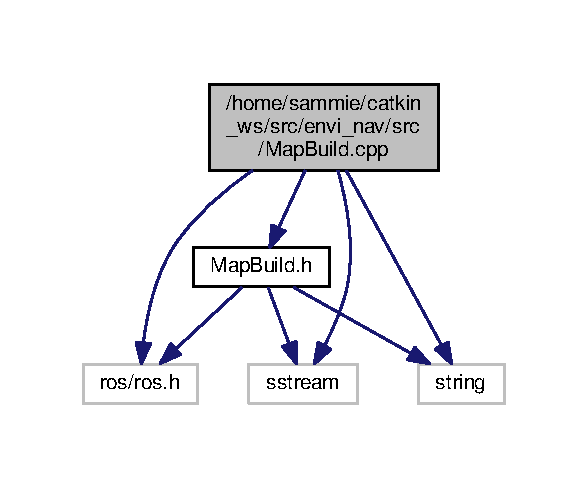
\includegraphics[width=282pt]{MapBuild_8cpp__incl}
\end{center}
\end{figure}


\subsection{Detailed Description}
Saves the map generated by the navigation demo. 

\begin{DoxyAuthor}{Author}
Samantha Johnson 
\end{DoxyAuthor}
\begin{DoxyDate}{Date}
December 15, 2017  B\+SD 3-\/\+Clause License 
\end{DoxyDate}
\begin{DoxyCopyright}{Copyright}
(c) 2017, Samantha Johnson All rights reserved.
\end{DoxyCopyright}
Redistribution and use in source and binary forms, with or without modification, are permitted provided that the following conditions are met\+:

Redistributions of source code must retain the above copyright notice, this list of conditions and the following disclaimer.

Redistributions in binary form must reproduce the above copyright notice, this list of conditions and the following disclaimer in the documentation and/or other materials provided with the distribution.

Neither the name of the copyright holder nor the names of its contributors may be used to endorse or promote products derived from this software without specific prior written permission.

T\+H\+IS S\+O\+F\+T\+W\+A\+RE IS P\+R\+O\+V\+I\+D\+ED BY T\+HE C\+O\+P\+Y\+R\+I\+G\+HT H\+O\+L\+D\+E\+RS A\+ND C\+O\+N\+T\+R\+I\+B\+U\+T\+O\+RS \char`\"{}\+A\+S I\+S\char`\"{} A\+ND A\+NY E\+X\+P\+R\+E\+SS OR I\+M\+P\+L\+I\+ED W\+A\+R\+R\+A\+N\+T\+I\+ES, I\+N\+C\+L\+U\+D\+I\+NG, B\+UT N\+OT L\+I\+M\+I\+T\+ED TO, T\+HE I\+M\+P\+L\+I\+ED W\+A\+R\+R\+A\+N\+T\+I\+ES OF M\+E\+R\+C\+H\+A\+N\+T\+A\+B\+I\+L\+I\+TY A\+ND F\+I\+T\+N\+E\+SS F\+OR A P\+A\+R\+T\+I\+C\+U\+L\+AR P\+U\+R\+P\+O\+SE A\+RE D\+I\+S\+C\+L\+A\+I\+M\+ED. IN NO E\+V\+E\+NT S\+H\+A\+LL T\+HE C\+O\+P\+Y\+R\+I\+G\+HT H\+O\+L\+D\+ER OR C\+O\+N\+T\+R\+I\+B\+U\+T\+O\+RS BE L\+I\+A\+B\+LE F\+OR A\+NY D\+I\+R\+E\+CT, I\+N\+D\+I\+R\+E\+CT, I\+N\+C\+I\+D\+E\+N\+T\+AL, S\+P\+E\+C\+I\+AL, E\+X\+E\+M\+P\+L\+A\+RY, OR C\+O\+N\+S\+E\+Q\+U\+E\+N\+T\+I\+AL D\+A\+M\+A\+G\+ES (I\+N\+C\+L\+U\+D\+I\+NG, B\+UT N\+OT L\+I\+M\+I\+T\+ED TO, P\+R\+O\+C\+U\+R\+E\+M\+E\+NT OF S\+U\+B\+S\+T\+I\+T\+U\+TE G\+O\+O\+DS OR S\+E\+R\+V\+I\+C\+ES; L\+O\+SS OF U\+SE, D\+A\+TA, OR P\+R\+O\+F\+I\+TS; OR B\+U\+S\+I\+N\+E\+SS I\+N\+T\+E\+R\+R\+U\+P\+T\+I\+ON) H\+O\+W\+E\+V\+ER C\+A\+U\+S\+ED A\+ND ON A\+NY T\+H\+E\+O\+RY OF L\+I\+A\+B\+I\+L\+I\+TY, W\+H\+E\+T\+H\+ER IN C\+O\+N\+T\+R\+A\+CT, S\+T\+R\+I\+CT L\+I\+A\+B\+I\+L\+I\+TY, OR T\+O\+RT (I\+N\+C\+L\+U\+D\+I\+NG N\+E\+G\+L\+I\+G\+E\+N\+CE OR O\+T\+H\+E\+R\+W\+I\+SE) A\+R\+I\+S\+I\+NG IN A\+NY W\+AY O\+UT OF T\+HE U\+SE OF T\+H\+IS S\+O\+F\+T\+W\+A\+RE, E\+V\+EN IF A\+D\+V\+I\+S\+ED OF T\+HE P\+O\+S\+S\+I\+B\+I\+L\+I\+TY OF S\+U\+CH D\+A\+M\+A\+GE.

Allows the user to save the map being built in the navigation demo by typing a simple command. 
\hypertarget{mapping__demo_8cpp}{}\section{/home/sammie/catkin\+\_\+ws/src/envi\+\_\+nav/src/mapping\+\_\+demo.cpp File Reference}
\label{mapping__demo_8cpp}\index{/home/sammie/catkin\+\_\+ws/src/envi\+\_\+nav/src/mapping\+\_\+demo.\+cpp@{/home/sammie/catkin\+\_\+ws/src/envi\+\_\+nav/src/mapping\+\_\+demo.\+cpp}}


Gives instructions for building the navigation map.  


{\ttfamily \#include $<$ros/ros.\+h$>$}\\*
{\ttfamily \#include \char`\"{}Map\+Build.\+h\char`\"{}}\\*
{\ttfamily \#include $<$sstream$>$}\\*
{\ttfamily \#include $<$string$>$}\\*
Include dependency graph for mapping\+\_\+demo.\+cpp\+:\nopagebreak
\begin{figure}[H]
\begin{center}
\leavevmode
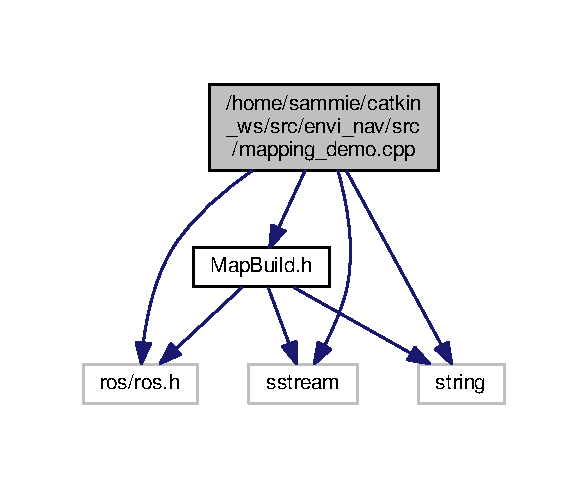
\includegraphics[width=282pt]{mapping__demo_8cpp__incl}
\end{center}
\end{figure}
\subsection*{Functions}
\begin{DoxyCompactItemize}
\item 
int {\bfseries main} (int argc, char $\ast$$\ast$argv)\hypertarget{mapping__demo_8cpp_a3c04138a5bfe5d72780bb7e82a18e627}{}\label{mapping__demo_8cpp_a3c04138a5bfe5d72780bb7e82a18e627}

\end{DoxyCompactItemize}


\subsection{Detailed Description}
Gives instructions for building the navigation map. 

\begin{DoxyAuthor}{Author}
Samantha Johnson 
\end{DoxyAuthor}
\begin{DoxyDate}{Date}
December 15, 2017  B\+SD 3-\/\+Clause License 
\end{DoxyDate}
\begin{DoxyCopyright}{Copyright}
(c) 2017, Samantha Johnson All rights reserved.
\end{DoxyCopyright}
Redistribution and use in source and binary forms, with or without modification, are permitted provided that the following conditions are met\+:

Redistributions of source code must retain the above copyright notice, this list of conditions and the following disclaimer.

Redistributions in binary form must reproduce the above copyright notice, this list of conditions and the following disclaimer in the documentation and/or other materials provided with the distribution.

Neither the name of the copyright holder nor the names of its contributors may be used to endorse or promote products derived from this software without specific prior written permission.

T\+H\+IS S\+O\+F\+T\+W\+A\+RE IS P\+R\+O\+V\+I\+D\+ED BY T\+HE C\+O\+P\+Y\+R\+I\+G\+HT H\+O\+L\+D\+E\+RS A\+ND C\+O\+N\+T\+R\+I\+B\+U\+T\+O\+RS \char`\"{}\+A\+S I\+S\char`\"{} A\+ND A\+NY E\+X\+P\+R\+E\+SS OR I\+M\+P\+L\+I\+ED W\+A\+R\+R\+A\+N\+T\+I\+ES, I\+N\+C\+L\+U\+D\+I\+NG, B\+UT N\+OT L\+I\+M\+I\+T\+ED TO, T\+HE I\+M\+P\+L\+I\+ED W\+A\+R\+R\+A\+N\+T\+I\+ES OF M\+E\+R\+C\+H\+A\+N\+T\+A\+B\+I\+L\+I\+TY A\+ND F\+I\+T\+N\+E\+SS F\+OR A P\+A\+R\+T\+I\+C\+U\+L\+AR P\+U\+R\+P\+O\+SE A\+RE D\+I\+S\+C\+L\+A\+I\+M\+ED. IN NO E\+V\+E\+NT S\+H\+A\+LL T\+HE C\+O\+P\+Y\+R\+I\+G\+HT H\+O\+L\+D\+ER OR C\+O\+N\+T\+R\+I\+B\+U\+T\+O\+RS BE L\+I\+A\+B\+LE F\+OR A\+NY D\+I\+R\+E\+CT, I\+N\+D\+I\+R\+E\+CT, I\+N\+C\+I\+D\+E\+N\+T\+AL, S\+P\+E\+C\+I\+AL, E\+X\+E\+M\+P\+L\+A\+RY, OR C\+O\+N\+S\+E\+Q\+U\+E\+N\+T\+I\+AL D\+A\+M\+A\+G\+ES (I\+N\+C\+L\+U\+D\+I\+NG, B\+UT N\+OT L\+I\+M\+I\+T\+ED TO, P\+R\+O\+C\+U\+R\+E\+M\+E\+NT OF S\+U\+B\+S\+T\+I\+T\+U\+TE G\+O\+O\+DS OR S\+E\+R\+V\+I\+C\+ES; L\+O\+SS OF U\+SE, D\+A\+TA, OR P\+R\+O\+F\+I\+TS; OR B\+U\+S\+I\+N\+E\+SS I\+N\+T\+E\+R\+R\+U\+P\+T\+I\+ON) H\+O\+W\+E\+V\+ER C\+A\+U\+S\+ED A\+ND ON A\+NY T\+H\+E\+O\+RY OF L\+I\+A\+B\+I\+L\+I\+TY, W\+H\+E\+T\+H\+ER IN C\+O\+N\+T\+R\+A\+CT, S\+T\+R\+I\+CT L\+I\+A\+B\+I\+L\+I\+TY, OR T\+O\+RT (I\+N\+C\+L\+U\+D\+I\+NG N\+E\+G\+L\+I\+G\+E\+N\+CE OR O\+T\+H\+E\+R\+W\+I\+SE) A\+R\+I\+S\+I\+NG IN A\+NY W\+AY O\+UT OF T\+HE U\+SE OF T\+H\+IS S\+O\+F\+T\+W\+A\+RE, E\+V\+EN IF A\+D\+V\+I\+S\+ED OF T\+HE P\+O\+S\+S\+I\+B\+I\+L\+I\+TY OF S\+U\+CH D\+A\+M\+A\+GE.

Provides detailed instructions for building the map that is used with the navigation demo. 
\hypertarget{RRTPlanner_8cpp}{}\section{/home/sammie/catkin\+\_\+ws/src/envi\+\_\+nav/src/\+R\+R\+T\+Planner.cpp File Reference}
\label{RRTPlanner_8cpp}\index{/home/sammie/catkin\+\_\+ws/src/envi\+\_\+nav/src/\+R\+R\+T\+Planner.\+cpp@{/home/sammie/catkin\+\_\+ws/src/envi\+\_\+nav/src/\+R\+R\+T\+Planner.\+cpp}}


Global path planner implementing the R\+RT algorithm.  


{\ttfamily \#include \char`\"{}R\+R\+T\+Planner.\+h\char`\"{}}\\*
{\ttfamily \#include \char`\"{}R\+R\+T\+Planner\+Helper.\+h\char`\"{}}\\*
{\ttfamily \#include $<$ros/ros.\+h$>$}\\*
{\ttfamily \#include $<$costmap\+\_\+2d/costmap\+\_\+2d\+\_\+ros.\+h$>$}\\*
{\ttfamily \#include $<$costmap\+\_\+2d/costmap\+\_\+2d.\+h$>$}\\*
{\ttfamily \#include $<$nav\+\_\+core/base\+\_\+global\+\_\+planner.\+h$>$}\\*
{\ttfamily \#include $<$geometry\+\_\+msgs/\+Pose\+Stamped.\+h$>$}\\*
{\ttfamily \#include $<$pluginlib/class\+\_\+list\+\_\+macros.\+h$>$}\\*
{\ttfamily \#include $<$algorithm$>$}\\*
{\ttfamily \#include $<$vector$>$}\\*
Include dependency graph for R\+R\+T\+Planner.\+cpp\+:\nopagebreak
\begin{figure}[H]
\begin{center}
\leavevmode
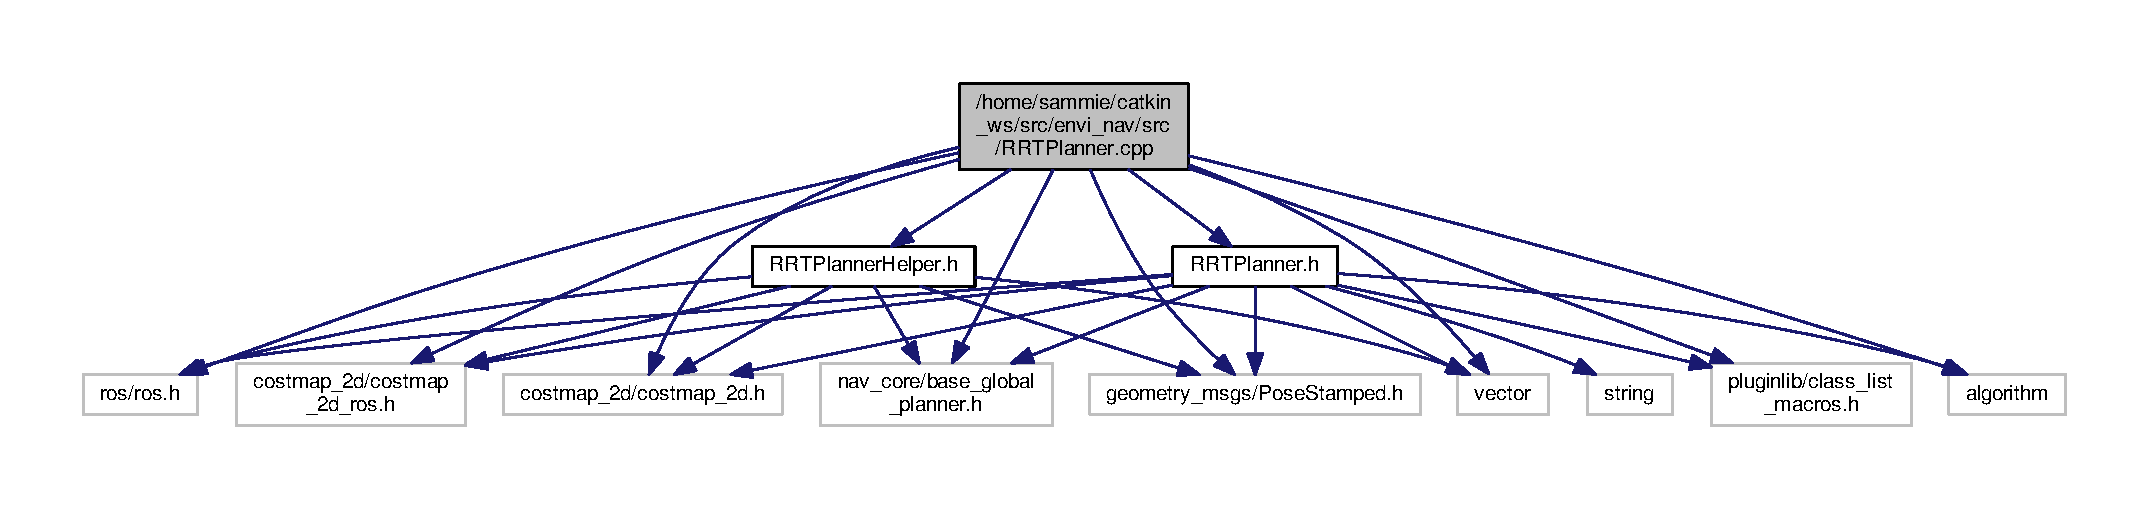
\includegraphics[width=350pt]{RRTPlanner_8cpp__incl}
\end{center}
\end{figure}


\subsection{Detailed Description}
Global path planner implementing the R\+RT algorithm. 

\begin{DoxyAuthor}{Author}
Samantha Johnson 
\end{DoxyAuthor}
\begin{DoxyDate}{Date}
December 15, 2017  B\+SD 3-\/\+Clause License 
\end{DoxyDate}
\begin{DoxyCopyright}{Copyright}
(c) 2017, Samantha Johnson All rights reserved.
\end{DoxyCopyright}
Redistribution and use in source and binary forms, with or without modification, are permitted provided that the following conditions are met\+:

Redistributions of source code must retain the above copyright notice, this list of conditions and the following disclaimer.

Redistributions in binary form must reproduce the above copyright notice, this list of conditions and the following disclaimer in the documentation and/or other materials provided with the distribution.

Neither the name of the copyright holder nor the names of its contributors may be used to endorse or promote products derived from this software without specific prior written permission.

T\+H\+IS S\+O\+F\+T\+W\+A\+RE IS P\+R\+O\+V\+I\+D\+ED BY T\+HE C\+O\+P\+Y\+R\+I\+G\+HT H\+O\+L\+D\+E\+RS A\+ND C\+O\+N\+T\+R\+I\+B\+U\+T\+O\+RS \char`\"{}\+A\+S I\+S\char`\"{} A\+ND A\+NY E\+X\+P\+R\+E\+SS OR I\+M\+P\+L\+I\+ED W\+A\+R\+R\+A\+N\+T\+I\+ES, I\+N\+C\+L\+U\+D\+I\+NG, B\+UT N\+OT L\+I\+M\+I\+T\+ED TO, T\+HE I\+M\+P\+L\+I\+ED W\+A\+R\+R\+A\+N\+T\+I\+ES OF M\+E\+R\+C\+H\+A\+N\+T\+A\+B\+I\+L\+I\+TY A\+ND F\+I\+T\+N\+E\+SS F\+OR A P\+A\+R\+T\+I\+C\+U\+L\+AR P\+U\+R\+P\+O\+SE A\+RE D\+I\+S\+C\+L\+A\+I\+M\+ED. IN NO E\+V\+E\+NT S\+H\+A\+LL T\+HE C\+O\+P\+Y\+R\+I\+G\+HT H\+O\+L\+D\+ER OR C\+O\+N\+T\+R\+I\+B\+U\+T\+O\+RS BE L\+I\+A\+B\+LE F\+OR A\+NY D\+I\+R\+E\+CT, I\+N\+D\+I\+R\+E\+CT, I\+N\+C\+I\+D\+E\+N\+T\+AL, S\+P\+E\+C\+I\+AL, E\+X\+E\+M\+P\+L\+A\+RY, OR C\+O\+N\+S\+E\+Q\+U\+E\+N\+T\+I\+AL D\+A\+M\+A\+G\+ES (I\+N\+C\+L\+U\+D\+I\+NG, B\+UT N\+OT L\+I\+M\+I\+T\+ED TO, P\+R\+O\+C\+U\+R\+E\+M\+E\+NT OF S\+U\+B\+S\+T\+I\+T\+U\+TE G\+O\+O\+DS OR S\+E\+R\+V\+I\+C\+ES; L\+O\+SS OF U\+SE, D\+A\+TA, OR P\+R\+O\+F\+I\+TS; OR B\+U\+S\+I\+N\+E\+SS I\+N\+T\+E\+R\+R\+U\+P\+T\+I\+ON) H\+O\+W\+E\+V\+ER C\+A\+U\+S\+ED A\+ND ON A\+NY T\+H\+E\+O\+RY OF L\+I\+A\+B\+I\+L\+I\+TY, W\+H\+E\+T\+H\+ER IN C\+O\+N\+T\+R\+A\+CT, S\+T\+R\+I\+CT L\+I\+A\+B\+I\+L\+I\+TY, OR T\+O\+RT (I\+N\+C\+L\+U\+D\+I\+NG N\+E\+G\+L\+I\+G\+E\+N\+CE OR O\+T\+H\+E\+R\+W\+I\+SE) A\+R\+I\+S\+I\+NG IN A\+NY W\+AY O\+UT OF T\+HE U\+SE OF T\+H\+IS S\+O\+F\+T\+W\+A\+RE, E\+V\+EN IF A\+D\+V\+I\+S\+ED OF T\+HE P\+O\+S\+S\+I\+B\+I\+L\+I\+TY OF S\+U\+CH D\+A\+M\+A\+GE.

This plugin was created to interface with the nav\+\_\+core/base\+\_\+global\+\_\+planner framework and replace the default global planner used in the navigation stack. This plugin uses an R\+RT algorithm which generates a path by creating a tree full of random nodes that are connected to their nearest node neighbor if the path is clear. Once the goal is reached by the tree, the planner returns a path which is a connection of the nodes in the tree that traverse from start to goal. 
\hypertarget{RRTPlannerHelper_8cpp}{}\section{/home/sammie/catkin\+\_\+ws/src/envi\+\_\+nav/src/\+R\+R\+T\+Planner\+Helper.cpp File Reference}
\label{RRTPlannerHelper_8cpp}\index{/home/sammie/catkin\+\_\+ws/src/envi\+\_\+nav/src/\+R\+R\+T\+Planner\+Helper.\+cpp@{/home/sammie/catkin\+\_\+ws/src/envi\+\_\+nav/src/\+R\+R\+T\+Planner\+Helper.\+cpp}}


Global path planner implementing the R\+RT algorithm.  


{\ttfamily \#include \char`\"{}R\+R\+T\+Planner\+Helper.\+h\char`\"{}}\\*
{\ttfamily \#include $<$ros/ros.\+h$>$}\\*
{\ttfamily \#include $<$costmap\+\_\+2d/costmap\+\_\+2d\+\_\+ros.\+h$>$}\\*
{\ttfamily \#include $<$costmap\+\_\+2d/costmap\+\_\+2d.\+h$>$}\\*
{\ttfamily \#include $<$nav\+\_\+core/base\+\_\+global\+\_\+planner.\+h$>$}\\*
{\ttfamily \#include $<$geometry\+\_\+msgs/\+Pose\+Stamped.\+h$>$}\\*
{\ttfamily \#include $<$algorithm$>$}\\*
{\ttfamily \#include $<$vector$>$}\\*
Include dependency graph for R\+R\+T\+Planner\+Helper.\+cpp\+:\nopagebreak
\begin{figure}[H]
\begin{center}
\leavevmode
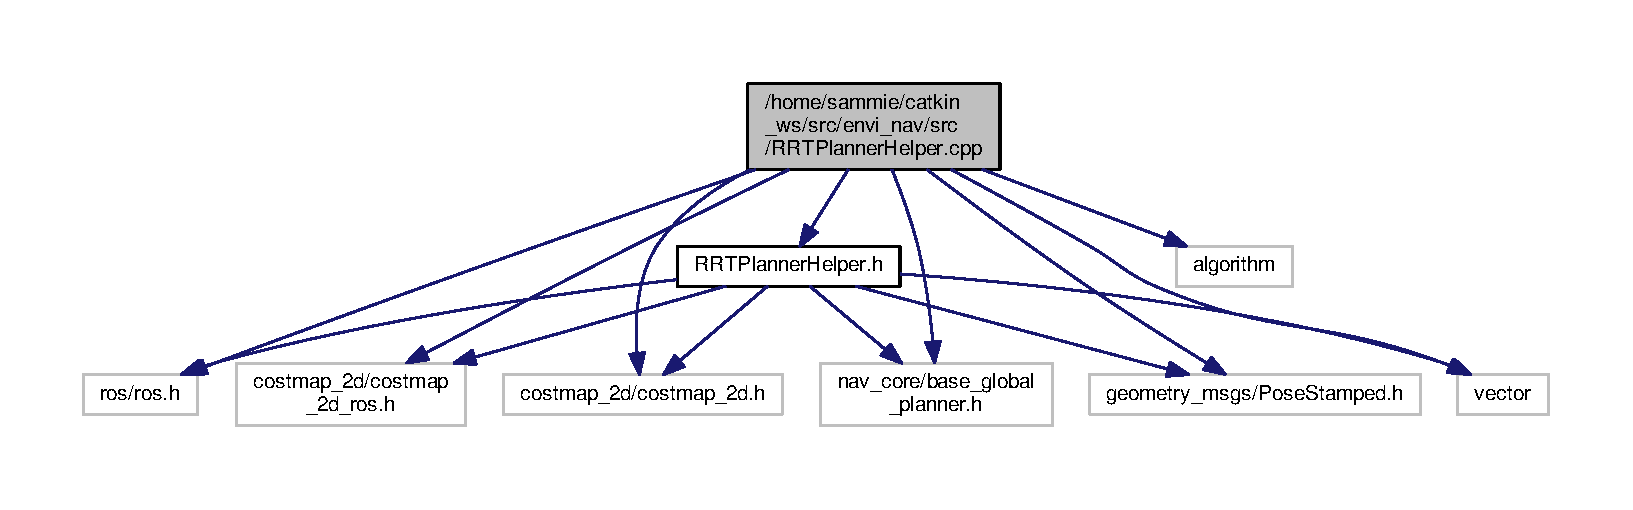
\includegraphics[width=350pt]{RRTPlannerHelper_8cpp__incl}
\end{center}
\end{figure}


\subsection{Detailed Description}
Global path planner implementing the R\+RT algorithm. 

\begin{DoxyAuthor}{Author}
Samantha Johnson 
\end{DoxyAuthor}
\begin{DoxyDate}{Date}
December 15, 2017  B\+SD 3-\/\+Clause License 
\end{DoxyDate}
\begin{DoxyCopyright}{Copyright}
(c) 2017, Samantha Johnson All rights reserved.
\end{DoxyCopyright}
Redistribution and use in source and binary forms, with or without modification, are permitted provided that the following conditions are met\+:

Redistributions of source code must retain the above copyright notice, this list of conditions and the following disclaimer.

Redistributions in binary form must reproduce the above copyright notice, this list of conditions and the following disclaimer in the documentation and/or other materials provided with the distribution.

Neither the name of the copyright holder nor the names of its contributors may be used to endorse or promote products derived from this software without specific prior written permission.

T\+H\+IS S\+O\+F\+T\+W\+A\+RE IS P\+R\+O\+V\+I\+D\+ED BY T\+HE C\+O\+P\+Y\+R\+I\+G\+HT H\+O\+L\+D\+E\+RS A\+ND C\+O\+N\+T\+R\+I\+B\+U\+T\+O\+RS \char`\"{}\+A\+S I\+S\char`\"{} A\+ND A\+NY E\+X\+P\+R\+E\+SS OR I\+M\+P\+L\+I\+ED W\+A\+R\+R\+A\+N\+T\+I\+ES, I\+N\+C\+L\+U\+D\+I\+NG, B\+UT N\+OT L\+I\+M\+I\+T\+ED TO, T\+HE I\+M\+P\+L\+I\+ED W\+A\+R\+R\+A\+N\+T\+I\+ES OF M\+E\+R\+C\+H\+A\+N\+T\+A\+B\+I\+L\+I\+TY A\+ND F\+I\+T\+N\+E\+SS F\+OR A P\+A\+R\+T\+I\+C\+U\+L\+AR P\+U\+R\+P\+O\+SE A\+RE D\+I\+S\+C\+L\+A\+I\+M\+ED. IN NO E\+V\+E\+NT S\+H\+A\+LL T\+HE C\+O\+P\+Y\+R\+I\+G\+HT H\+O\+L\+D\+ER OR C\+O\+N\+T\+R\+I\+B\+U\+T\+O\+RS BE L\+I\+A\+B\+LE F\+OR A\+NY D\+I\+R\+E\+CT, I\+N\+D\+I\+R\+E\+CT, I\+N\+C\+I\+D\+E\+N\+T\+AL, S\+P\+E\+C\+I\+AL, E\+X\+E\+M\+P\+L\+A\+RY, OR C\+O\+N\+S\+E\+Q\+U\+E\+N\+T\+I\+AL D\+A\+M\+A\+G\+ES (I\+N\+C\+L\+U\+D\+I\+NG, B\+UT N\+OT L\+I\+M\+I\+T\+ED TO, P\+R\+O\+C\+U\+R\+E\+M\+E\+NT OF S\+U\+B\+S\+T\+I\+T\+U\+TE G\+O\+O\+DS OR S\+E\+R\+V\+I\+C\+ES; L\+O\+SS OF U\+SE, D\+A\+TA, OR P\+R\+O\+F\+I\+TS; OR B\+U\+S\+I\+N\+E\+SS I\+N\+T\+E\+R\+R\+U\+P\+T\+I\+ON) H\+O\+W\+E\+V\+ER C\+A\+U\+S\+ED A\+ND ON A\+NY T\+H\+E\+O\+RY OF L\+I\+A\+B\+I\+L\+I\+TY, W\+H\+E\+T\+H\+ER IN C\+O\+N\+T\+R\+A\+CT, S\+T\+R\+I\+CT L\+I\+A\+B\+I\+L\+I\+TY, OR T\+O\+RT (I\+N\+C\+L\+U\+D\+I\+NG N\+E\+G\+L\+I\+G\+E\+N\+CE OR O\+T\+H\+E\+R\+W\+I\+SE) A\+R\+I\+S\+I\+NG IN A\+NY W\+AY O\+UT OF T\+HE U\+SE OF T\+H\+IS S\+O\+F\+T\+W\+A\+RE, E\+V\+EN IF A\+D\+V\+I\+S\+ED OF T\+HE P\+O\+S\+S\+I\+B\+I\+L\+I\+TY OF S\+U\+CH D\+A\+M\+A\+GE.

This class was created to perform the calculations for the \hyperlink{classRRTPlanner}{R\+R\+T\+Planner} plugin. This class implements an R\+RT algorithm which generates a path by creating a tree full of random nodes that are connected to their nearest node neighbor if the path is clear. Once the goal is reached by the tree, the planner returns a path which is a connection of the nodes in the tree that traverse from start to goal. 
\hypertarget{EnviNavTests_8cpp}{}\section{/home/sammie/catkin\+\_\+ws/src/envi\+\_\+nav/test/\+Envi\+Nav\+Tests.cpp File Reference}
\label{EnviNavTests_8cpp}\index{/home/sammie/catkin\+\_\+ws/src/envi\+\_\+nav/test/\+Envi\+Nav\+Tests.\+cpp@{/home/sammie/catkin\+\_\+ws/src/envi\+\_\+nav/test/\+Envi\+Nav\+Tests.\+cpp}}


Tests for R\+RT Planning algorithm.  


{\ttfamily \#include $<$geometry\+\_\+msgs/\+Pose\+Stamped.\+h$>$}\\*
{\ttfamily \#include $<$costmap\+\_\+2d/costmap\+\_\+2d.\+h$>$}\\*
{\ttfamily \#include $<$costmap\+\_\+2d/costmap\+\_\+2d\+\_\+ros.\+h$>$}\\*
{\ttfamily \#include $<$tf/transform\+\_\+listener.\+h$>$}\\*
{\ttfamily \#include $<$pluginlib/class\+\_\+loader.\+h$>$}\\*
{\ttfamily \#include $<$nav\+\_\+core/base\+\_\+global\+\_\+planner.\+h$>$}\\*
{\ttfamily \#include $<$gtest/gtest.\+h$>$}\\*
{\ttfamily \#include $<$ros/ros.\+h$>$}\\*
{\ttfamily \#include \char`\"{}R\+R\+T\+Planner\+Helper.\+h\char`\"{}}\\*
{\ttfamily \#include $<$vector$>$}\\*
Include dependency graph for Envi\+Nav\+Tests.\+cpp\+:\nopagebreak
\begin{figure}[H]
\begin{center}
\leavevmode
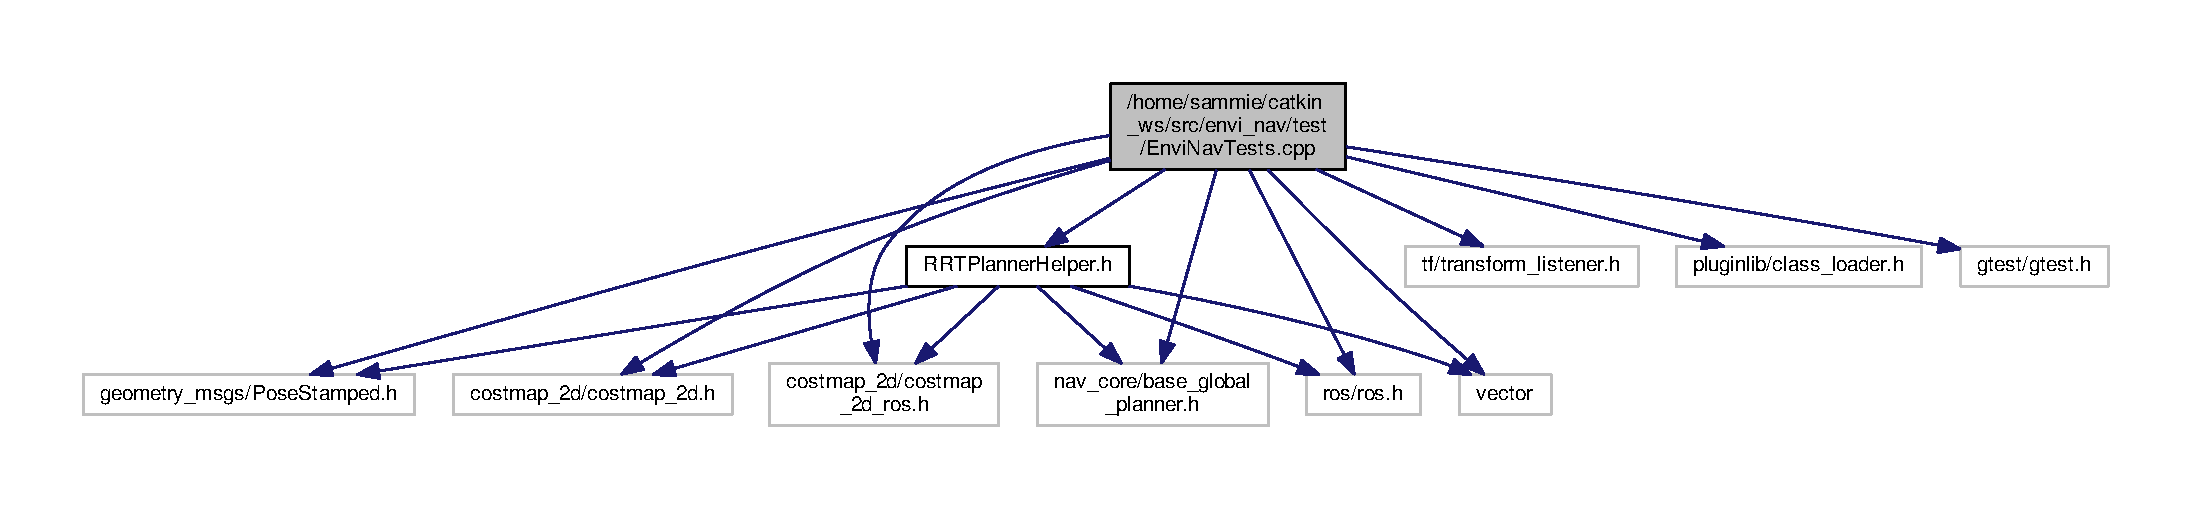
\includegraphics[width=350pt]{EnviNavTests_8cpp__incl}
\end{center}
\end{figure}
\subsection*{Classes}
\begin{DoxyCompactItemize}
\item 
class \hyperlink{classRRTPlannerTester}{R\+R\+T\+Planner\+Tester}
\end{DoxyCompactItemize}
\subsection*{Functions}
\begin{DoxyCompactItemize}
\item 
{\bfseries T\+E\+ST} (R\+R\+T\+Planner\+Helper\+\_\+test, test\+Random\+Node\+Returned\+In\+Map)\hypertarget{EnviNavTests_8cpp_a30d771ebff6f9a2f4ee2644148ba2d17}{}\label{EnviNavTests_8cpp_a30d771ebff6f9a2f4ee2644148ba2d17}

\item 
{\bfseries T\+E\+ST} (R\+R\+T\+Planner\+\_\+test, test\+Nearest\+Node\+Returned\+From\+Tree\+Graph)\hypertarget{EnviNavTests_8cpp_a353d72db1768549c293348dfd4321418}{}\label{EnviNavTests_8cpp_a353d72db1768549c293348dfd4321418}

\item 
{\bfseries T\+E\+ST} (R\+R\+T\+Planner\+\_\+test, test\+Path\+Between\+Nodes\+Is\+Safe)\hypertarget{EnviNavTests_8cpp_a18cda9b5208b0db48f3c6106262c1464}{}\label{EnviNavTests_8cpp_a18cda9b5208b0db48f3c6106262c1464}

\item 
{\bfseries T\+E\+ST} (R\+R\+T\+Planner\+\_\+test, test\+Path\+To\+Goal\+Is\+Safe)\hypertarget{EnviNavTests_8cpp_a00a680f40a43d54add2136b2d9c281c9}{}\label{EnviNavTests_8cpp_a00a680f40a43d54add2136b2d9c281c9}

\item 
{\bfseries T\+E\+ST} (R\+R\+T\+Planner\+\_\+test, test\+Build\+Plan\+Is\+Correct)\hypertarget{EnviNavTests_8cpp_aadaae3148b63ed1051ee75013b8ed9f2}{}\label{EnviNavTests_8cpp_aadaae3148b63ed1051ee75013b8ed9f2}

\item 
int {\bfseries main} (int argc, char $\ast$$\ast$argv)\hypertarget{EnviNavTests_8cpp_a3c04138a5bfe5d72780bb7e82a18e627}{}\label{EnviNavTests_8cpp_a3c04138a5bfe5d72780bb7e82a18e627}

\end{DoxyCompactItemize}


\subsection{Detailed Description}
Tests for R\+RT Planning algorithm. 

\begin{DoxyAuthor}{Author}
Samantha Johnson 
\end{DoxyAuthor}
\begin{DoxyDate}{Date}
December 15, 2017  B\+SD 3-\/\+Clause License 
\end{DoxyDate}
\begin{DoxyCopyright}{Copyright}
(c) 2017, Samantha Johnson All rights reserved.
\end{DoxyCopyright}
Redistribution and use in source and binary forms, with or without modification, are permitted provided that the following conditions are met\+:

Redistributions of source code must retain the above copyright notice, this list of conditions and the following disclaimer.

Redistributions in binary form must reproduce the above copyright notice, this list of conditions and the following disclaimer in the documentation and/or other materials provided with the distribution.

Neither the name of the copyright holder nor the names of its contributors may be used to endorse or promote products derived from this software without specific prior written permission.

T\+H\+IS S\+O\+F\+T\+W\+A\+RE IS P\+R\+O\+V\+I\+D\+ED BY T\+HE C\+O\+P\+Y\+R\+I\+G\+HT H\+O\+L\+D\+E\+RS A\+ND C\+O\+N\+T\+R\+I\+B\+U\+T\+O\+RS \char`\"{}\+A\+S I\+S\char`\"{} A\+ND A\+NY E\+X\+P\+R\+E\+SS OR I\+M\+P\+L\+I\+ED W\+A\+R\+R\+A\+N\+T\+I\+ES, I\+N\+C\+L\+U\+D\+I\+NG, B\+UT N\+OT L\+I\+M\+I\+T\+ED TO, T\+HE I\+M\+P\+L\+I\+ED W\+A\+R\+R\+A\+N\+T\+I\+ES OF M\+E\+R\+C\+H\+A\+N\+T\+A\+B\+I\+L\+I\+TY A\+ND F\+I\+T\+N\+E\+SS F\+OR A P\+A\+R\+T\+I\+C\+U\+L\+AR P\+U\+R\+P\+O\+SE A\+RE D\+I\+S\+C\+L\+A\+I\+M\+ED. IN NO E\+V\+E\+NT S\+H\+A\+LL T\+HE C\+O\+P\+Y\+R\+I\+G\+HT H\+O\+L\+D\+ER OR C\+O\+N\+T\+R\+I\+B\+U\+T\+O\+RS BE L\+I\+A\+B\+LE F\+OR A\+NY D\+I\+R\+E\+CT, I\+N\+D\+I\+R\+E\+CT, I\+N\+C\+I\+D\+E\+N\+T\+AL, S\+P\+E\+C\+I\+AL, E\+X\+E\+M\+P\+L\+A\+RY, OR C\+O\+N\+S\+E\+Q\+U\+E\+N\+T\+I\+AL D\+A\+M\+A\+G\+ES (I\+N\+C\+L\+U\+D\+I\+NG, B\+UT N\+OT L\+I\+M\+I\+T\+ED TO, P\+R\+O\+C\+U\+R\+E\+M\+E\+NT OF S\+U\+B\+S\+T\+I\+T\+U\+TE G\+O\+O\+DS OR S\+E\+R\+V\+I\+C\+ES; L\+O\+SS OF U\+SE, D\+A\+TA, OR P\+R\+O\+F\+I\+TS; OR B\+U\+S\+I\+N\+E\+SS I\+N\+T\+E\+R\+R\+U\+P\+T\+I\+ON) H\+O\+W\+E\+V\+ER C\+A\+U\+S\+ED A\+ND ON A\+NY T\+H\+E\+O\+RY OF L\+I\+A\+B\+I\+L\+I\+TY, W\+H\+E\+T\+H\+ER IN C\+O\+N\+T\+R\+A\+CT, S\+T\+R\+I\+CT L\+I\+A\+B\+I\+L\+I\+TY, OR T\+O\+RT (I\+N\+C\+L\+U\+D\+I\+NG N\+E\+G\+L\+I\+G\+E\+N\+CE OR O\+T\+H\+E\+R\+W\+I\+SE) A\+R\+I\+S\+I\+NG IN A\+NY W\+AY O\+UT OF T\+HE U\+SE OF T\+H\+IS S\+O\+F\+T\+W\+A\+RE, E\+V\+EN IF A\+D\+V\+I\+S\+ED OF T\+HE P\+O\+S\+S\+I\+B\+I\+L\+I\+TY OF S\+U\+CH D\+A\+M\+A\+GE.

Tests for the R\+RT algorithm used as a global path planner plugin to the navigation stack 
%--- End generated contents ---

% Index
\backmatter
\newpage
\phantomsection
\clearemptydoublepage
\addcontentsline{toc}{chapter}{Index}
\printindex

\end{document}
